% $Author$
% $Date$
% $Revision$
% $Id$

% HISTORY:
% 2007-10-29 - Oscar started chapter
% 2007-11-30 - Oscar first draft
% 2007-12-07 - Orla Greevy reviewed
% 2007-12-09 - Lukas Renggli reviewed
% 2008-01-11 - Andrew revised
% 2009-04-17 - Fabrizio Perin reviewed
% 2009-04-18 - Jorge Ressia reviewed
% 2009-05-06 - Oscar converted to Pharo; fixed review comments
% 2011-05-29 - Rafael Luque translated to spanish
%=================================================================
\ifx\wholebook\relax\else
% --------------------------------------------
% Lulu:
	\documentclass[a4paper,10pt,twoside]{book}
	\usepackage[
		papersize={6.13in,9.21in},
		hmargin={.75in,.75in},
		vmargin={.75in,1in},
		ignoreheadfoot
	]{geometry}
	% $Author$
% $Date$
% $Revision$

% HISTORY:
% 2006-10-31 - Oscar code macros
% ...

%=============================================================
% NB: documentclass must be set in main document.
% Allows book to be generated in multiple formats.
%=============================================================
%:Packages
\usepackage[T1]{fontenc}  %%%%%% really important to get the code directly in the text!
\usepackage{lmodern}
%\usepackage[scaled=0.85]{bookmanx} % needs another scale factor if used with \renewcommand{\sfdefault}{cmbr}
\usepackage{palatino}
\usepackage[scaled=0.85]{helvet}
\usepackage{microtype}
\usepackage{graphicx}
\usepackage{theorem}
\usepackage[english]{babel}
% ON: pdfsync breaks the use of p{width} for tabular columns!
\ifdefined\usepdfsync\usepackage{pdfsync}\fi % Requires texlive 2007
%=============================================================
%:More packages
%Stef should check which ones are used!
%\usepackage{picinpar}
%\usepackage{layout}
%\usepackage{color}
%\usepackage{enum}
%\usepackage{a4wide}
% \usepackage{fancyhdr}
\usepackage{ifthen}
\usepackage{float}
\usepackage{longtable}
\usepackage{makeidx}
\usepackage[nottoc]{tocbibind}
\usepackage{multicol}
\usepackage{booktabs}	% book-style tables
\usepackage{topcapt}	% enables \topcaption
\usepackage{multirow}
\usepackage{tabularx}
%\usepackage[bottom]{footmisc}
\usepackage{xspace}
\usepackage{alltt}
\usepackage{amssymb,textcomp}
\usepackage[usenames,dvipsnames]{color}
%\usepackage{colortbl}
\usepackage[hang]{subfigure}\makeatletter\def\p@subfigure{\thefigure\,}\makeatother
\usepackage{rotating}
\usepackage{enumitem}	% apb: allows more control over tags in enumerations
\usepackage{verbatim}     % for comment environment
\usepackage{varioref}	% for page references that work
\labelformat{footnote}{\thechapter--#1} % to distinguish citations from jurabib
\usepackage{needspace}
\usepackage{isodateo} % enable \isodate
\usepackage[newparttoc]{titlesec}
\usepackage{titletoc}
\usepackage{wrapfig}
\usepackage[
	super,
	citefull=first,
	authorformat={allreversed,and},
	titleformat={commasep,italic}
]{jurabib} % citations as footnotes
\usepackage[
	colorlinks=true,
	linkcolor=black,
	urlcolor=black,
	citecolor=black
]{hyperref}   % should come last
%=============================================================
%:PDF version
\pdfminorversion=3 % Set PDF to 1.3 for Lulu
%=============================================================
%:URL style
\makeatletter
\def\url@leostyle{%
  \@ifundefined{selectfont}{\def\UrlFont{\sf}}{\def\UrlFont{\sffamily}}}
\makeatother
% Now actually use the newly defined style.
\urlstyle{leo}
%=============================================================
%:Booleans
\newboolean{lulu}
\setboolean{lulu}{false}
\newcommand{\ifluluelse}[2]{\ifthenelse{\boolean{lulu}}{#1}{#2}}
%=============================================================
%:Names
\newcommand{\SUnit}{SUnit\xspace}
\newcommand{\sunit}{SUnit\xspace}
\newcommand{\xUnit}{$x$Unit\xspace}
\newcommand{\JUnit}{JUnit\xspace}
\newcommand{\st}{Smalltalk\xspace}
\newcommand{\pharo}{Pharo\xspace} % Use this, not \Pharo
%\newcommand{\sqmap}{SqueakMap\xspace}
\newcommand{\squeak}{Squeak\xspace} % use this, not \Squeak or \sq
\newcommand{\sqsrc}{SqueakSource\xspace}
\newcommand{\sbe}{\url{http://SqueakByExample.org}\xspace}
\newcommand{\pharoweb}{\url{http://pharo-project.org}\xspace}
\newcommand{\pbe}{\url{http://PharoByExample.org}\xspace}
\newcommand{\sba}{\url{http://SquareBracketAssociates.org}\xspace}
\newcommand{\bam}{\lct{Bounc\-ing\-Atoms\-Morph}\xspace}
%=============================================================
%:Markup macros for proof-reading
\usepackage[normalem]{ulem} % for \sout
\usepackage{xcolor}
\newcommand{\ra}{$\rightarrow$}
\newcommand{\ugh}[1]{\textcolor{red}{\uwave{#1}}} % please rephrase
\newcommand{\ins}[1]{\textcolor{blue}{\uline{#1}}} % please insert
\newcommand{\del}[1]{\textcolor{red}{\sout{#1}}} % please delete
\newcommand{\chg}[2]{\textcolor{red}{\sout{#1}}{\ra}\textcolor{blue}{\uline{#2}}} % please change
%=============================================================
%:Editorial comment macros
%\newcommand{\nnbb}[2]{
%    % \fbox{\bfseries\sffamily\scriptsize#1}
%    \fcolorbox{gray}{yellow}{\bfseries\sffamily\scriptsize#1}
%    {\sf\small$\blacktriangleright$\textit{#2}$\blacktriangleleft$}
%   }
\newcommand{\yellowbox}[1]{\fcolorbox{gray}{yellow}{\bfseries\sffamily\scriptsize#1}}
\newcommand{\triangles}[1]{{\sf\small$\blacktriangleright$\textit{#1}$\blacktriangleleft$}}
\newcommand{\nnbb}[2]{\yellowbox{#1} \triangles{#2}}
\newcommand{\fix}{\yellowbox{FIX!}}
\newcommand{\here}{\yellowbox{CONTINUE HERE!}}
% editor macros
\newcommand{\ab}[1]{\nnbb{Andrew}{#1}} % Black
\newcommand{\sd}[1]{\nnbb{St\'{e}f}{#1}} % Ducasse
\newcommand{\md}[1]{\nnbb{Marcus}{#1}} % Denker
\newcommand{\on}[1]{\nnbb{Oscar}{#1}} % Nierstrasz
\newcommand{\damien}[1]{\nnbb{Damien}{#1}} % Pollet
\newcommand{\lr}[1]{\nnbb{Lukas}{#1}} % Renggli
\newcommand{\orla}[1]{\nnbb{Orla}{#1}} % Greevy
\newcommand{\alex}[1]{\nnbb{Alex}{#1}} % Bergel
\newcommand{\alx}[1]{\nnbb{Alex}{#1}} % Bergel
\newcommand{\dr}[1]{\nnbb{David}{#1}} % Roethlisberger
\newcommand{\ja}[1]{\nnbb{Jannik}{#1}} % Laval
\newcommand{\jr}[1]{\nnbb{Jorge}{#1}} % Ressia
\newcommand{\fp}[1]{\nnbb{Fabrizio}{#1}} % Perin
\newcommand{\michael}[1]{\nnbb{Michael}{#1}} % Davies
\newcommand{\ew}[1]{\nnbb{Erwann}{#1}} % Wernli
\newcommand{\mb}[1]{\nnbb{Martial}{#1}} % Boniou
\newcommand{\hw}[1]{\nnbb{Hernan}{#1}} % Wilkinson
%=============================================================
%:Abbreviation macros
\newcommand{\ie}{\emph{i.e.},\xspace}
\newcommand{\eg}{\emph{e.g.},\xspace}
\newcommand{\etc}{etc.\xspace}
%=============================================================
%:Cross reference macros
\newcommand{\charef}[1]{Chapter~\ref{cha:#1}\xspace}
\newcommand{\secref}[1]{Section~\ref{sec:#1}\xspace}
\newcommand{\figref}[1]{Figure~\ref{fig:#1}\xspace}
\newcommand{\Figref}[1]{Figure~\ref{fig:#1}\xspace}
\newcommand{\appref}[1]{Appendix~\ref{app:#1}\xspace}
\newcommand{\tabref}[1]{Table~\ref{tab:#1}\xspace}
\newcommand{\faqref}[1]{FAQ~\ref{faq:#1}, p.~\pageref{faq:#1}\xspace}
% APB: I removed trailing \xspace commands from these macros because
% \xspace mostly doesn't work.  If you want a space after your
% references, type one!
% ON: xspace has always worked just fine for me!  Please leave them in.
%
\newcommand{\ruleref}[1]{\ref{rule:#1}\xspace}
%
\newcommand{\egref}[1]{example~\ref{eg:#1}\xspace}
\newcommand{\Egref}[1]{Example~\ref{eg:#1}\xspace}
%
\newcommand{\scrref}[1]{script~\ref{scr:#1}\xspace}
\newcommand{\Scrref}[1]{Script~\ref{scr:#1}\xspace}
\newcommand{\tscrref}[1]{the script~\ref{scr:#1}\xspace}
\newcommand{\Tscrref}[1]{The script~\ref{scr:#1}\xspace}
%
\newcommand{\mthref}[1]{method~\ref{mth:#1}\xspace}
\newcommand{\mthsref}[1]{methods~\ref{mth:#1}\xspace}
\newcommand{\Mthref}[1]{Method~\ref{mth:#1}\xspace}
\newcommand{\tmthref}[1]{the method~\ref{mth:#1}\xspace}
\newcommand{\Tmthref}[1]{The method~\ref{mth:#1}\xspace}
%
\newcommand{\clsref}[1]{class~\ref{cls:#1}\xspace}
\newcommand{\tclsref}[1]{the class~\ref{cls:#1}\xspace}
\newcommand{\Tclsref}[1]{The class~\ref{cls:#1}\xspace}

\newcommand{\chalabel}[1]{\label{cha:#1}}
\newcommand{\seclabel}[1]{\label{sec:#1}}
\newcommand{\figlabel}[1]{\label{fig:#1}}
\newcommand{\tablabel}[1]{\label{tab:#1}}
\newcommand{\rulelabel}[1]{\label{rule:#1}}
\newcommand{\eglabel}[1]{\label{eg:#1}}
\newcommand{\scrlabel}[1]{\label{scr:#1}}
\newcommand{\mthlabel}[1]{\label{mth:#1}}
\newcommand{\clslabel}[1]{\label{cls:#1}}
\newcommand{\faqlabel}[1]{\label{faq:#1}}
%=============================================================
%:Menu item macro
% for menu items, so we can change our minds on how to print them! (apb)
\definecolor{lightgray}{gray}{0.89}
\newcommand{\menu}[1]{{%
	\setlength{\fboxsep}{0pt}%
	\colorbox{lightgray}{{{\upshape\sffamily\strut \,#1\,}}}}}
\newcommand{\link}[1]{{%
	\fontfamily{lmr}\selectfont
 	\upshape{\sffamily \underline{#1}}}}
% For submenu items:
\newcommand{\go}{\,$\triangleright$\,}
% \newcommand{\go}{\,$\blacktriangleright$\,}
% For keyboard shortcuts:
%\newcommand{\short}[1]{\mbox{$\langle${\sc CMD}$\rangle$-#1}\xspace}
\newcommand{\short}[1]{\mbox{{\sc cmd}\hspace{0.08em}--\hspace{0.09em}#1}\xspace}
% For buttons:
\newcommand{\button}[1]{{%
	\setlength{\fboxsep}{0pt}%
	\fbox{{\upshape\sffamily\strut \,#1\,}}}}
% NB: The button macro does not work within captions -- incompatible with xcolor package :-(
\newcommand{\toolsflap}{\textit{Tools} flap\xspace}
%=============================================================
%:Mouse clicks
\newcommand{\click}{click\xspace} % RED
\newcommand{\actclick}{action-click\xspace} % YELLOW
\newcommand{\metaclick}{meta-click\xspace} % BLUE
\newcommand{\Click}{Click\xspace} % RED
\newcommand{\Actclick}{Action-click\xspace} % YELLOW
\newcommand{\Metaclick}{Meta-click\xspace} % BLUE
%=============================================================
%:ToSh macros
\newboolean{tosh}
\setboolean{tosh}{false}
\newcommand{\iftoshelse}[2]{\ifthenelse{\boolean{tosh}}{#1}{#2}}
%=============================================================
%:ToSh colors
%\newcommand{\highlightcolor}{\color{blue!65}}
%\newcommand{\boxcolor}{\color{gray!25}}
\newcommand{\highlight}[1]{\textcolor{blue!65}{#1}}
%\newcommand{\codecolor}{\color{blue!65}}
%%\setlength{\fboxrule}{2pt}
%\newcommand{\asPict}[1]{%
%	{\Large\highlight{#1}}}
%=============================================================
%:Reader cues (do this)
%
% Indicate something the reader should try out.
% \newcommand{\dothisicon}{\raisebox{-.5ex}{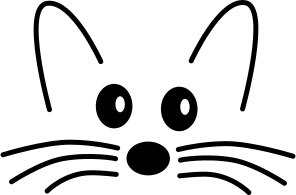
\includegraphics[width=1.4em]{squeak-logo}}}
\iftoshelse{
	\usepackage{marginnote}
		\renewcommand*{\marginfont}{\footnotesize}
	\newcommand{\vartriangleout}{\ifthenelse{\isodd{\thepage}}{\vartriangleright}{\vartriangleleft}}
	\newcommand{\dothisicon}{\fcolorbox{blue!65}{white}{\highlight{$\vartriangleout$}}}
	\newcommand{\dothis}[1]{%
		\noindent\par\noindent
		{\reversemarginpar
			\marginnote{\fcolorbox{blue!65}{white}{\highlight{$\vartriangleout$}}}}
		%\MarginLabel{do this}
		\noindent\emph{#1}
		\nopagebreak}
}{
	\newcommand{\dothisicon}{\raisebox{-.5ex}{
\includegraphics[height=1.2em]{pharo}}}
	\newcommand{\dothis}[1]{%
		\medskip
		\noindent\dothisicon
		\ifx#1\empty\else\quad\emph{#1}\fi
		\par\smallskip\nopagebreak}
}
%===> NEW VERSION <===
% NB: To use this in an individual chapter, you must set:
%\graphicspath{{figures/} {../figures/}}
% at the head of the chapter.  Don't forget the final /
%=============================================================
%:Reader hints (hint)
%
% Indicates a non-obvious consequence 
\newcommand{\hint}[1]{\vspace{1ex}\noindent\fbox{\textsc{Hint}} \emph{#1}}
%=================================================================
% graphics for Morphic handles
\newcommand{\grabHandle}{\raisebox{-0.2ex}{
\includegraphics[width=1em]{blackHandle}}}
\newcommand{\moveHandle}{\raisebox{-0.2ex}{
\includegraphics[width=1em]{moveHandle}}}
\newcommand{\debugHandle}{\raisebox{-0.2ex}{
\includegraphics[width=1em]{debugHandle}}}
%=============================================================
%:Highlighting Important stuff (doublebox)
%
% From Seaside book ...
\newsavebox{\SavedText}
\newlength{\InnerBoxRule}\setlength{\InnerBoxRule}{.75\fboxrule}
\newlength{\OuterBoxRule}\setlength{\OuterBoxRule}{1.5\fboxrule}
\newlength{\BoxSeparation}\setlength{\BoxSeparation}{1.5\fboxrule}
\addtolength{\BoxSeparation}{.5pt}
\newlength{\SaveBoxSep}\setlength{\SaveBoxSep}{2\fboxsep}
%
\newenvironment{doublebox}{\begin{lrbox}{\SavedText}
    \begin{minipage}{.75\textwidth}}
    {\end{minipage}\end{lrbox}\begin{center}
    \setlength{\fboxsep}{\BoxSeparation}\setlength{\fboxrule}{\OuterBoxRule}
    \fbox{\setlength{\fboxsep}{\SaveBoxSep}\setlength{\fboxrule}{\InnerBoxRule}%
      \fbox{\usebox{\SavedText}}}
  \end{center}}
% Use this:
\newcommand{\important}[1]{\begin{doublebox}#1\end{doublebox}}
%=============================================================
%:Section depth
\setcounter{secnumdepth}{2}
%% for this to happen start the file with
%\ifx\wholebook\relax\else
%% $Author$
% $Date$
% $Revision$

% HISTORY:
% 2006-10-31 - Oscar code macros
% ...

%=============================================================
% NB: documentclass must be set in main document.
% Allows book to be generated in multiple formats.
%=============================================================
%:Packages
\usepackage[T1]{fontenc}  %%%%%% really important to get the code directly in the text!
\usepackage{lmodern}
%\usepackage[scaled=0.85]{bookmanx} % needs another scale factor if used with \renewcommand{\sfdefault}{cmbr}
\usepackage{palatino}
\usepackage[scaled=0.85]{helvet}
\usepackage{microtype}
\usepackage{graphicx}
\usepackage{theorem}
\usepackage[english]{babel}
% ON: pdfsync breaks the use of p{width} for tabular columns!
\ifdefined\usepdfsync\usepackage{pdfsync}\fi % Requires texlive 2007
%=============================================================
%:More packages
%Stef should check which ones are used!
%\usepackage{picinpar}
%\usepackage{layout}
%\usepackage{color}
%\usepackage{enum}
%\usepackage{a4wide}
% \usepackage{fancyhdr}
\usepackage{ifthen}
\usepackage{float}
\usepackage{longtable}
\usepackage{makeidx}
\usepackage[nottoc]{tocbibind}
\usepackage{multicol}
\usepackage{booktabs}	% book-style tables
\usepackage{topcapt}	% enables \topcaption
\usepackage{multirow}
\usepackage{tabularx}
%\usepackage[bottom]{footmisc}
\usepackage{xspace}
\usepackage{alltt}
\usepackage{amssymb,textcomp}
\usepackage[usenames,dvipsnames]{color}
%\usepackage{colortbl}
\usepackage[hang]{subfigure}\makeatletter\def\p@subfigure{\thefigure\,}\makeatother
\usepackage{rotating}
\usepackage{enumitem}	% apb: allows more control over tags in enumerations
\usepackage{verbatim}     % for comment environment
\usepackage{varioref}	% for page references that work
\labelformat{footnote}{\thechapter--#1} % to distinguish citations from jurabib
\usepackage{needspace}
\usepackage{isodateo} % enable \isodate
\usepackage[newparttoc]{titlesec}
\usepackage{titletoc}
\usepackage{wrapfig}
\usepackage[
	super,
	citefull=first,
	authorformat={allreversed,and},
	titleformat={commasep,italic}
]{jurabib} % citations as footnotes
\usepackage[
	colorlinks=true,
	linkcolor=black,
	urlcolor=black,
	citecolor=black
]{hyperref}   % should come last
%=============================================================
%:PDF version
\pdfminorversion=3 % Set PDF to 1.3 for Lulu
%=============================================================
%:URL style
\makeatletter
\def\url@leostyle{%
  \@ifundefined{selectfont}{\def\UrlFont{\sf}}{\def\UrlFont{\sffamily}}}
\makeatother
% Now actually use the newly defined style.
\urlstyle{leo}
%=============================================================
%:Booleans
\newboolean{lulu}
\setboolean{lulu}{false}
\newcommand{\ifluluelse}[2]{\ifthenelse{\boolean{lulu}}{#1}{#2}}
%=============================================================
%:Names
\newcommand{\SUnit}{SUnit\xspace}
\newcommand{\sunit}{SUnit\xspace}
\newcommand{\xUnit}{$x$Unit\xspace}
\newcommand{\JUnit}{JUnit\xspace}
\newcommand{\st}{Smalltalk\xspace}
\newcommand{\pharo}{Pharo\xspace} % Use this, not \Pharo
%\newcommand{\sqmap}{SqueakMap\xspace}
\newcommand{\squeak}{Squeak\xspace} % use this, not \Squeak or \sq
\newcommand{\sqsrc}{SqueakSource\xspace}
\newcommand{\sbe}{\url{http://SqueakByExample.org}\xspace}
\newcommand{\pharoweb}{\url{http://pharo-project.org}\xspace}
\newcommand{\pbe}{\url{http://PharoByExample.org}\xspace}
\newcommand{\sba}{\url{http://SquareBracketAssociates.org}\xspace}
\newcommand{\bam}{\lct{Bounc\-ing\-Atoms\-Morph}\xspace}
%=============================================================
%:Markup macros for proof-reading
\usepackage[normalem]{ulem} % for \sout
\usepackage{xcolor}
\newcommand{\ra}{$\rightarrow$}
\newcommand{\ugh}[1]{\textcolor{red}{\uwave{#1}}} % please rephrase
\newcommand{\ins}[1]{\textcolor{blue}{\uline{#1}}} % please insert
\newcommand{\del}[1]{\textcolor{red}{\sout{#1}}} % please delete
\newcommand{\chg}[2]{\textcolor{red}{\sout{#1}}{\ra}\textcolor{blue}{\uline{#2}}} % please change
%=============================================================
%:Editorial comment macros
%\newcommand{\nnbb}[2]{
%    % \fbox{\bfseries\sffamily\scriptsize#1}
%    \fcolorbox{gray}{yellow}{\bfseries\sffamily\scriptsize#1}
%    {\sf\small$\blacktriangleright$\textit{#2}$\blacktriangleleft$}
%   }
\newcommand{\yellowbox}[1]{\fcolorbox{gray}{yellow}{\bfseries\sffamily\scriptsize#1}}
\newcommand{\triangles}[1]{{\sf\small$\blacktriangleright$\textit{#1}$\blacktriangleleft$}}
\newcommand{\nnbb}[2]{\yellowbox{#1} \triangles{#2}}
\newcommand{\fix}{\yellowbox{FIX!}}
\newcommand{\here}{\yellowbox{CONTINUE HERE!}}
% editor macros
\newcommand{\ab}[1]{\nnbb{Andrew}{#1}} % Black
\newcommand{\sd}[1]{\nnbb{St\'{e}f}{#1}} % Ducasse
\newcommand{\md}[1]{\nnbb{Marcus}{#1}} % Denker
\newcommand{\on}[1]{\nnbb{Oscar}{#1}} % Nierstrasz
\newcommand{\damien}[1]{\nnbb{Damien}{#1}} % Pollet
\newcommand{\lr}[1]{\nnbb{Lukas}{#1}} % Renggli
\newcommand{\orla}[1]{\nnbb{Orla}{#1}} % Greevy
\newcommand{\alex}[1]{\nnbb{Alex}{#1}} % Bergel
\newcommand{\alx}[1]{\nnbb{Alex}{#1}} % Bergel
\newcommand{\dr}[1]{\nnbb{David}{#1}} % Roethlisberger
\newcommand{\ja}[1]{\nnbb{Jannik}{#1}} % Laval
\newcommand{\jr}[1]{\nnbb{Jorge}{#1}} % Ressia
\newcommand{\fp}[1]{\nnbb{Fabrizio}{#1}} % Perin
\newcommand{\michael}[1]{\nnbb{Michael}{#1}} % Davies
\newcommand{\ew}[1]{\nnbb{Erwann}{#1}} % Wernli
\newcommand{\mb}[1]{\nnbb{Martial}{#1}} % Boniou
\newcommand{\hw}[1]{\nnbb{Hernan}{#1}} % Wilkinson
%=============================================================
%:Abbreviation macros
\newcommand{\ie}{\emph{i.e.},\xspace}
\newcommand{\eg}{\emph{e.g.},\xspace}
\newcommand{\etc}{etc.\xspace}
%=============================================================
%:Cross reference macros
\newcommand{\charef}[1]{Chapter~\ref{cha:#1}\xspace}
\newcommand{\secref}[1]{Section~\ref{sec:#1}\xspace}
\newcommand{\figref}[1]{Figure~\ref{fig:#1}\xspace}
\newcommand{\Figref}[1]{Figure~\ref{fig:#1}\xspace}
\newcommand{\appref}[1]{Appendix~\ref{app:#1}\xspace}
\newcommand{\tabref}[1]{Table~\ref{tab:#1}\xspace}
\newcommand{\faqref}[1]{FAQ~\ref{faq:#1}, p.~\pageref{faq:#1}\xspace}
% APB: I removed trailing \xspace commands from these macros because
% \xspace mostly doesn't work.  If you want a space after your
% references, type one!
% ON: xspace has always worked just fine for me!  Please leave them in.
%
\newcommand{\ruleref}[1]{\ref{rule:#1}\xspace}
%
\newcommand{\egref}[1]{example~\ref{eg:#1}\xspace}
\newcommand{\Egref}[1]{Example~\ref{eg:#1}\xspace}
%
\newcommand{\scrref}[1]{script~\ref{scr:#1}\xspace}
\newcommand{\Scrref}[1]{Script~\ref{scr:#1}\xspace}
\newcommand{\tscrref}[1]{the script~\ref{scr:#1}\xspace}
\newcommand{\Tscrref}[1]{The script~\ref{scr:#1}\xspace}
%
\newcommand{\mthref}[1]{method~\ref{mth:#1}\xspace}
\newcommand{\mthsref}[1]{methods~\ref{mth:#1}\xspace}
\newcommand{\Mthref}[1]{Method~\ref{mth:#1}\xspace}
\newcommand{\tmthref}[1]{the method~\ref{mth:#1}\xspace}
\newcommand{\Tmthref}[1]{The method~\ref{mth:#1}\xspace}
%
\newcommand{\clsref}[1]{class~\ref{cls:#1}\xspace}
\newcommand{\tclsref}[1]{the class~\ref{cls:#1}\xspace}
\newcommand{\Tclsref}[1]{The class~\ref{cls:#1}\xspace}

\newcommand{\chalabel}[1]{\label{cha:#1}}
\newcommand{\seclabel}[1]{\label{sec:#1}}
\newcommand{\figlabel}[1]{\label{fig:#1}}
\newcommand{\tablabel}[1]{\label{tab:#1}}
\newcommand{\rulelabel}[1]{\label{rule:#1}}
\newcommand{\eglabel}[1]{\label{eg:#1}}
\newcommand{\scrlabel}[1]{\label{scr:#1}}
\newcommand{\mthlabel}[1]{\label{mth:#1}}
\newcommand{\clslabel}[1]{\label{cls:#1}}
\newcommand{\faqlabel}[1]{\label{faq:#1}}
%=============================================================
%:Menu item macro
% for menu items, so we can change our minds on how to print them! (apb)
\definecolor{lightgray}{gray}{0.89}
\newcommand{\menu}[1]{{%
	\setlength{\fboxsep}{0pt}%
	\colorbox{lightgray}{{{\upshape\sffamily\strut \,#1\,}}}}}
\newcommand{\link}[1]{{%
	\fontfamily{lmr}\selectfont
 	\upshape{\sffamily \underline{#1}}}}
% For submenu items:
\newcommand{\go}{\,$\triangleright$\,}
% \newcommand{\go}{\,$\blacktriangleright$\,}
% For keyboard shortcuts:
%\newcommand{\short}[1]{\mbox{$\langle${\sc CMD}$\rangle$-#1}\xspace}
\newcommand{\short}[1]{\mbox{{\sc cmd}\hspace{0.08em}--\hspace{0.09em}#1}\xspace}
% For buttons:
\newcommand{\button}[1]{{%
	\setlength{\fboxsep}{0pt}%
	\fbox{{\upshape\sffamily\strut \,#1\,}}}}
% NB: The button macro does not work within captions -- incompatible with xcolor package :-(
\newcommand{\toolsflap}{\textit{Tools} flap\xspace}
%=============================================================
%:Mouse clicks
\newcommand{\click}{click\xspace} % RED
\newcommand{\actclick}{action-click\xspace} % YELLOW
\newcommand{\metaclick}{meta-click\xspace} % BLUE
\newcommand{\Click}{Click\xspace} % RED
\newcommand{\Actclick}{Action-click\xspace} % YELLOW
\newcommand{\Metaclick}{Meta-click\xspace} % BLUE
%=============================================================
%:ToSh macros
\newboolean{tosh}
\setboolean{tosh}{false}
\newcommand{\iftoshelse}[2]{\ifthenelse{\boolean{tosh}}{#1}{#2}}
%=============================================================
%:ToSh colors
%\newcommand{\highlightcolor}{\color{blue!65}}
%\newcommand{\boxcolor}{\color{gray!25}}
\newcommand{\highlight}[1]{\textcolor{blue!65}{#1}}
%\newcommand{\codecolor}{\color{blue!65}}
%%\setlength{\fboxrule}{2pt}
%\newcommand{\asPict}[1]{%
%	{\Large\highlight{#1}}}
%=============================================================
%:Reader cues (do this)
%
% Indicate something the reader should try out.
% \newcommand{\dothisicon}{\raisebox{-.5ex}{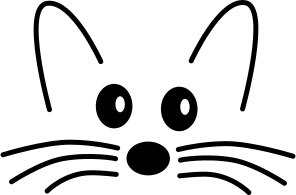
\includegraphics[width=1.4em]{squeak-logo}}}
\iftoshelse{
	\usepackage{marginnote}
		\renewcommand*{\marginfont}{\footnotesize}
	\newcommand{\vartriangleout}{\ifthenelse{\isodd{\thepage}}{\vartriangleright}{\vartriangleleft}}
	\newcommand{\dothisicon}{\fcolorbox{blue!65}{white}{\highlight{$\vartriangleout$}}}
	\newcommand{\dothis}[1]{%
		\noindent\par\noindent
		{\reversemarginpar
			\marginnote{\fcolorbox{blue!65}{white}{\highlight{$\vartriangleout$}}}}
		%\MarginLabel{do this}
		\noindent\emph{#1}
		\nopagebreak}
}{
	\newcommand{\dothisicon}{\raisebox{-.5ex}{
\includegraphics[height=1.2em]{pharo}}}
	\newcommand{\dothis}[1]{%
		\medskip
		\noindent\dothisicon
		\ifx#1\empty\else\quad\emph{#1}\fi
		\par\smallskip\nopagebreak}
}
%===> NEW VERSION <===
% NB: To use this in an individual chapter, you must set:
%\graphicspath{{figures/} {../figures/}}
% at the head of the chapter.  Don't forget the final /
%=============================================================
%:Reader hints (hint)
%
% Indicates a non-obvious consequence 
\newcommand{\hint}[1]{\vspace{1ex}\noindent\fbox{\textsc{Hint}} \emph{#1}}
%=================================================================
% graphics for Morphic handles
\newcommand{\grabHandle}{\raisebox{-0.2ex}{
\includegraphics[width=1em]{blackHandle}}}
\newcommand{\moveHandle}{\raisebox{-0.2ex}{
\includegraphics[width=1em]{moveHandle}}}
\newcommand{\debugHandle}{\raisebox{-0.2ex}{
\includegraphics[width=1em]{debugHandle}}}
%=============================================================
%:Highlighting Important stuff (doublebox)
%
% From Seaside book ...
\newsavebox{\SavedText}
\newlength{\InnerBoxRule}\setlength{\InnerBoxRule}{.75\fboxrule}
\newlength{\OuterBoxRule}\setlength{\OuterBoxRule}{1.5\fboxrule}
\newlength{\BoxSeparation}\setlength{\BoxSeparation}{1.5\fboxrule}
\addtolength{\BoxSeparation}{.5pt}
\newlength{\SaveBoxSep}\setlength{\SaveBoxSep}{2\fboxsep}
%
\newenvironment{doublebox}{\begin{lrbox}{\SavedText}
    \begin{minipage}{.75\textwidth}}
    {\end{minipage}\end{lrbox}\begin{center}
    \setlength{\fboxsep}{\BoxSeparation}\setlength{\fboxrule}{\OuterBoxRule}
    \fbox{\setlength{\fboxsep}{\SaveBoxSep}\setlength{\fboxrule}{\InnerBoxRule}%
      \fbox{\usebox{\SavedText}}}
  \end{center}}
% Use this:
\newcommand{\important}[1]{\begin{doublebox}#1\end{doublebox}}
%=============================================================
%:Section depth
\setcounter{secnumdepth}{2}
%% for this to happen start the file with
%\ifx\wholebook\relax\else
%% $Author$
% $Date$
% $Revision$

% HISTORY:
% 2006-10-31 - Oscar code macros
% ...

%=============================================================
% NB: documentclass must be set in main document.
% Allows book to be generated in multiple formats.
%=============================================================
%:Packages
\usepackage[T1]{fontenc}  %%%%%% really important to get the code directly in the text!
\usepackage{lmodern}
%\usepackage[scaled=0.85]{bookmanx} % needs another scale factor if used with \renewcommand{\sfdefault}{cmbr}
\usepackage{palatino}
\usepackage[scaled=0.85]{helvet}
\usepackage{microtype}
\usepackage{graphicx}
\usepackage{theorem}
\usepackage[english]{babel}
% ON: pdfsync breaks the use of p{width} for tabular columns!
\ifdefined\usepdfsync\usepackage{pdfsync}\fi % Requires texlive 2007
%=============================================================
%:More packages
%Stef should check which ones are used!
%\usepackage{picinpar}
%\usepackage{layout}
%\usepackage{color}
%\usepackage{enum}
%\usepackage{a4wide}
% \usepackage{fancyhdr}
\usepackage{ifthen}
\usepackage{float}
\usepackage{longtable}
\usepackage{makeidx}
\usepackage[nottoc]{tocbibind}
\usepackage{multicol}
\usepackage{booktabs}	% book-style tables
\usepackage{topcapt}	% enables \topcaption
\usepackage{multirow}
\usepackage{tabularx}
%\usepackage[bottom]{footmisc}
\usepackage{xspace}
\usepackage{alltt}
\usepackage{amssymb,textcomp}
\usepackage[usenames,dvipsnames]{color}
%\usepackage{colortbl}
\usepackage[hang]{subfigure}\makeatletter\def\p@subfigure{\thefigure\,}\makeatother
\usepackage{rotating}
\usepackage{enumitem}	% apb: allows more control over tags in enumerations
\usepackage{verbatim}     % for comment environment
\usepackage{varioref}	% for page references that work
\labelformat{footnote}{\thechapter--#1} % to distinguish citations from jurabib
\usepackage{needspace}
\usepackage{isodateo} % enable \isodate
\usepackage[newparttoc]{titlesec}
\usepackage{titletoc}
\usepackage{wrapfig}
\usepackage[
	super,
	citefull=first,
	authorformat={allreversed,and},
	titleformat={commasep,italic}
]{jurabib} % citations as footnotes
\usepackage[
	colorlinks=true,
	linkcolor=black,
	urlcolor=black,
	citecolor=black
]{hyperref}   % should come last
%=============================================================
%:PDF version
\pdfminorversion=3 % Set PDF to 1.3 for Lulu
%=============================================================
%:URL style
\makeatletter
\def\url@leostyle{%
  \@ifundefined{selectfont}{\def\UrlFont{\sf}}{\def\UrlFont{\sffamily}}}
\makeatother
% Now actually use the newly defined style.
\urlstyle{leo}
%=============================================================
%:Booleans
\newboolean{lulu}
\setboolean{lulu}{false}
\newcommand{\ifluluelse}[2]{\ifthenelse{\boolean{lulu}}{#1}{#2}}
%=============================================================
%:Names
\newcommand{\SUnit}{SUnit\xspace}
\newcommand{\sunit}{SUnit\xspace}
\newcommand{\xUnit}{$x$Unit\xspace}
\newcommand{\JUnit}{JUnit\xspace}
\newcommand{\st}{Smalltalk\xspace}
\newcommand{\pharo}{Pharo\xspace} % Use this, not \Pharo
%\newcommand{\sqmap}{SqueakMap\xspace}
\newcommand{\squeak}{Squeak\xspace} % use this, not \Squeak or \sq
\newcommand{\sqsrc}{SqueakSource\xspace}
\newcommand{\sbe}{\url{http://SqueakByExample.org}\xspace}
\newcommand{\pharoweb}{\url{http://pharo-project.org}\xspace}
\newcommand{\pbe}{\url{http://PharoByExample.org}\xspace}
\newcommand{\sba}{\url{http://SquareBracketAssociates.org}\xspace}
\newcommand{\bam}{\lct{Bounc\-ing\-Atoms\-Morph}\xspace}
%=============================================================
%:Markup macros for proof-reading
\usepackage[normalem]{ulem} % for \sout
\usepackage{xcolor}
\newcommand{\ra}{$\rightarrow$}
\newcommand{\ugh}[1]{\textcolor{red}{\uwave{#1}}} % please rephrase
\newcommand{\ins}[1]{\textcolor{blue}{\uline{#1}}} % please insert
\newcommand{\del}[1]{\textcolor{red}{\sout{#1}}} % please delete
\newcommand{\chg}[2]{\textcolor{red}{\sout{#1}}{\ra}\textcolor{blue}{\uline{#2}}} % please change
%=============================================================
%:Editorial comment macros
%\newcommand{\nnbb}[2]{
%    % \fbox{\bfseries\sffamily\scriptsize#1}
%    \fcolorbox{gray}{yellow}{\bfseries\sffamily\scriptsize#1}
%    {\sf\small$\blacktriangleright$\textit{#2}$\blacktriangleleft$}
%   }
\newcommand{\yellowbox}[1]{\fcolorbox{gray}{yellow}{\bfseries\sffamily\scriptsize#1}}
\newcommand{\triangles}[1]{{\sf\small$\blacktriangleright$\textit{#1}$\blacktriangleleft$}}
\newcommand{\nnbb}[2]{\yellowbox{#1} \triangles{#2}}
\newcommand{\fix}{\yellowbox{FIX!}}
\newcommand{\here}{\yellowbox{CONTINUE HERE!}}
% editor macros
\newcommand{\ab}[1]{\nnbb{Andrew}{#1}} % Black
\newcommand{\sd}[1]{\nnbb{St\'{e}f}{#1}} % Ducasse
\newcommand{\md}[1]{\nnbb{Marcus}{#1}} % Denker
\newcommand{\on}[1]{\nnbb{Oscar}{#1}} % Nierstrasz
\newcommand{\damien}[1]{\nnbb{Damien}{#1}} % Pollet
\newcommand{\lr}[1]{\nnbb{Lukas}{#1}} % Renggli
\newcommand{\orla}[1]{\nnbb{Orla}{#1}} % Greevy
\newcommand{\alex}[1]{\nnbb{Alex}{#1}} % Bergel
\newcommand{\alx}[1]{\nnbb{Alex}{#1}} % Bergel
\newcommand{\dr}[1]{\nnbb{David}{#1}} % Roethlisberger
\newcommand{\ja}[1]{\nnbb{Jannik}{#1}} % Laval
\newcommand{\jr}[1]{\nnbb{Jorge}{#1}} % Ressia
\newcommand{\fp}[1]{\nnbb{Fabrizio}{#1}} % Perin
\newcommand{\michael}[1]{\nnbb{Michael}{#1}} % Davies
\newcommand{\ew}[1]{\nnbb{Erwann}{#1}} % Wernli
\newcommand{\mb}[1]{\nnbb{Martial}{#1}} % Boniou
\newcommand{\hw}[1]{\nnbb{Hernan}{#1}} % Wilkinson
%=============================================================
%:Abbreviation macros
\newcommand{\ie}{\emph{i.e.},\xspace}
\newcommand{\eg}{\emph{e.g.},\xspace}
\newcommand{\etc}{etc.\xspace}
%=============================================================
%:Cross reference macros
\newcommand{\charef}[1]{Chapter~\ref{cha:#1}\xspace}
\newcommand{\secref}[1]{Section~\ref{sec:#1}\xspace}
\newcommand{\figref}[1]{Figure~\ref{fig:#1}\xspace}
\newcommand{\Figref}[1]{Figure~\ref{fig:#1}\xspace}
\newcommand{\appref}[1]{Appendix~\ref{app:#1}\xspace}
\newcommand{\tabref}[1]{Table~\ref{tab:#1}\xspace}
\newcommand{\faqref}[1]{FAQ~\ref{faq:#1}, p.~\pageref{faq:#1}\xspace}
% APB: I removed trailing \xspace commands from these macros because
% \xspace mostly doesn't work.  If you want a space after your
% references, type one!
% ON: xspace has always worked just fine for me!  Please leave them in.
%
\newcommand{\ruleref}[1]{\ref{rule:#1}\xspace}
%
\newcommand{\egref}[1]{example~\ref{eg:#1}\xspace}
\newcommand{\Egref}[1]{Example~\ref{eg:#1}\xspace}
%
\newcommand{\scrref}[1]{script~\ref{scr:#1}\xspace}
\newcommand{\Scrref}[1]{Script~\ref{scr:#1}\xspace}
\newcommand{\tscrref}[1]{the script~\ref{scr:#1}\xspace}
\newcommand{\Tscrref}[1]{The script~\ref{scr:#1}\xspace}
%
\newcommand{\mthref}[1]{method~\ref{mth:#1}\xspace}
\newcommand{\mthsref}[1]{methods~\ref{mth:#1}\xspace}
\newcommand{\Mthref}[1]{Method~\ref{mth:#1}\xspace}
\newcommand{\tmthref}[1]{the method~\ref{mth:#1}\xspace}
\newcommand{\Tmthref}[1]{The method~\ref{mth:#1}\xspace}
%
\newcommand{\clsref}[1]{class~\ref{cls:#1}\xspace}
\newcommand{\tclsref}[1]{the class~\ref{cls:#1}\xspace}
\newcommand{\Tclsref}[1]{The class~\ref{cls:#1}\xspace}

\newcommand{\chalabel}[1]{\label{cha:#1}}
\newcommand{\seclabel}[1]{\label{sec:#1}}
\newcommand{\figlabel}[1]{\label{fig:#1}}
\newcommand{\tablabel}[1]{\label{tab:#1}}
\newcommand{\rulelabel}[1]{\label{rule:#1}}
\newcommand{\eglabel}[1]{\label{eg:#1}}
\newcommand{\scrlabel}[1]{\label{scr:#1}}
\newcommand{\mthlabel}[1]{\label{mth:#1}}
\newcommand{\clslabel}[1]{\label{cls:#1}}
\newcommand{\faqlabel}[1]{\label{faq:#1}}
%=============================================================
%:Menu item macro
% for menu items, so we can change our minds on how to print them! (apb)
\definecolor{lightgray}{gray}{0.89}
\newcommand{\menu}[1]{{%
	\setlength{\fboxsep}{0pt}%
	\colorbox{lightgray}{{{\upshape\sffamily\strut \,#1\,}}}}}
\newcommand{\link}[1]{{%
	\fontfamily{lmr}\selectfont
 	\upshape{\sffamily \underline{#1}}}}
% For submenu items:
\newcommand{\go}{\,$\triangleright$\,}
% \newcommand{\go}{\,$\blacktriangleright$\,}
% For keyboard shortcuts:
%\newcommand{\short}[1]{\mbox{$\langle${\sc CMD}$\rangle$-#1}\xspace}
\newcommand{\short}[1]{\mbox{{\sc cmd}\hspace{0.08em}--\hspace{0.09em}#1}\xspace}
% For buttons:
\newcommand{\button}[1]{{%
	\setlength{\fboxsep}{0pt}%
	\fbox{{\upshape\sffamily\strut \,#1\,}}}}
% NB: The button macro does not work within captions -- incompatible with xcolor package :-(
\newcommand{\toolsflap}{\textit{Tools} flap\xspace}
%=============================================================
%:Mouse clicks
\newcommand{\click}{click\xspace} % RED
\newcommand{\actclick}{action-click\xspace} % YELLOW
\newcommand{\metaclick}{meta-click\xspace} % BLUE
\newcommand{\Click}{Click\xspace} % RED
\newcommand{\Actclick}{Action-click\xspace} % YELLOW
\newcommand{\Metaclick}{Meta-click\xspace} % BLUE
%=============================================================
%:ToSh macros
\newboolean{tosh}
\setboolean{tosh}{false}
\newcommand{\iftoshelse}[2]{\ifthenelse{\boolean{tosh}}{#1}{#2}}
%=============================================================
%:ToSh colors
%\newcommand{\highlightcolor}{\color{blue!65}}
%\newcommand{\boxcolor}{\color{gray!25}}
\newcommand{\highlight}[1]{\textcolor{blue!65}{#1}}
%\newcommand{\codecolor}{\color{blue!65}}
%%\setlength{\fboxrule}{2pt}
%\newcommand{\asPict}[1]{%
%	{\Large\highlight{#1}}}
%=============================================================
%:Reader cues (do this)
%
% Indicate something the reader should try out.
% \newcommand{\dothisicon}{\raisebox{-.5ex}{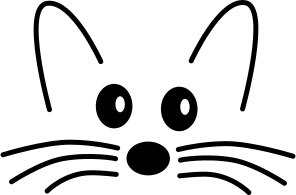
\includegraphics[width=1.4em]{squeak-logo}}}
\iftoshelse{
	\usepackage{marginnote}
		\renewcommand*{\marginfont}{\footnotesize}
	\newcommand{\vartriangleout}{\ifthenelse{\isodd{\thepage}}{\vartriangleright}{\vartriangleleft}}
	\newcommand{\dothisicon}{\fcolorbox{blue!65}{white}{\highlight{$\vartriangleout$}}}
	\newcommand{\dothis}[1]{%
		\noindent\par\noindent
		{\reversemarginpar
			\marginnote{\fcolorbox{blue!65}{white}{\highlight{$\vartriangleout$}}}}
		%\MarginLabel{do this}
		\noindent\emph{#1}
		\nopagebreak}
}{
	\newcommand{\dothisicon}{\raisebox{-.5ex}{
\includegraphics[height=1.2em]{pharo}}}
	\newcommand{\dothis}[1]{%
		\medskip
		\noindent\dothisicon
		\ifx#1\empty\else\quad\emph{#1}\fi
		\par\smallskip\nopagebreak}
}
%===> NEW VERSION <===
% NB: To use this in an individual chapter, you must set:
%\graphicspath{{figures/} {../figures/}}
% at the head of the chapter.  Don't forget the final /
%=============================================================
%:Reader hints (hint)
%
% Indicates a non-obvious consequence 
\newcommand{\hint}[1]{\vspace{1ex}\noindent\fbox{\textsc{Hint}} \emph{#1}}
%=================================================================
% graphics for Morphic handles
\newcommand{\grabHandle}{\raisebox{-0.2ex}{
\includegraphics[width=1em]{blackHandle}}}
\newcommand{\moveHandle}{\raisebox{-0.2ex}{
\includegraphics[width=1em]{moveHandle}}}
\newcommand{\debugHandle}{\raisebox{-0.2ex}{
\includegraphics[width=1em]{debugHandle}}}
%=============================================================
%:Highlighting Important stuff (doublebox)
%
% From Seaside book ...
\newsavebox{\SavedText}
\newlength{\InnerBoxRule}\setlength{\InnerBoxRule}{.75\fboxrule}
\newlength{\OuterBoxRule}\setlength{\OuterBoxRule}{1.5\fboxrule}
\newlength{\BoxSeparation}\setlength{\BoxSeparation}{1.5\fboxrule}
\addtolength{\BoxSeparation}{.5pt}
\newlength{\SaveBoxSep}\setlength{\SaveBoxSep}{2\fboxsep}
%
\newenvironment{doublebox}{\begin{lrbox}{\SavedText}
    \begin{minipage}{.75\textwidth}}
    {\end{minipage}\end{lrbox}\begin{center}
    \setlength{\fboxsep}{\BoxSeparation}\setlength{\fboxrule}{\OuterBoxRule}
    \fbox{\setlength{\fboxsep}{\SaveBoxSep}\setlength{\fboxrule}{\InnerBoxRule}%
      \fbox{\usebox{\SavedText}}}
  \end{center}}
% Use this:
\newcommand{\important}[1]{\begin{doublebox}#1\end{doublebox}}
%=============================================================
%:Section depth
\setcounter{secnumdepth}{2}
%% for this to happen start the file with
%\ifx\wholebook\relax\else
%\input{../common.tex}
%\begin{document}
%\fi
% and terminate by
% \ifx\wholebook\relax\else\end{document}\fi

\DeclareGraphicsExtensions{.pdf, .jpg, .png}
%=============================================================
%:PDF setup
\hypersetup{
%   a4paper,
%   pdfstartview=FitV,
%   colorlinks,
%   linkcolor=darkblue,
%   citecolor=darkblue,
   pdftitle={Pharo by Example},
   pdfauthor={Andrew P. Black, St\'ephane Ducasse,	Oscar Nierstrasz,
Damien Pollet},
   pdfkeywords={Smalltalk, Squeak, Object-Oriented Programming, OOP},
   pdfsubject={Computer Science}
}
%=============================================================
%:Page layout and appearance
%
% \renewcommand{\headrulewidth}{0pt}
\renewcommand{\chaptermark}[1]{\markboth{#1}{}}
\renewcommand{\sectionmark}[1]{\markright{\thesection\ #1}}
\renewpagestyle{plain}[\small\itshape]{%
	\setheadrule{0pt}%
	\sethead[][][]{}{}{}%
	\setfoot[][][]{}{}{}}
\renewpagestyle{headings}[\small\itshape]{%
	\setheadrule{0pt}%
	\setmarks{chapter}{section}%
	\sethead[\thepage][][\chaptertitle]{\sectiontitle}{}{\thepage}%
	\setfoot[][][]{}{}{}}
%=============================================================
%:Title section setup and TOC numbering depth
\setcounter{secnumdepth}{1}
\setcounter{tocdepth}{1}
\titleformat{\part}[display]{\centering}{\huge\partname\ \thepart}{1em}{\Huge\textbf}[]
\titleformat{\chapter}[display]{}{\huge\chaptertitlename\ \thechapter}{1em}{\Huge\raggedright\textbf}[]
\titlecontents{part}[3pc]{%
		\pagebreak[2]\addvspace{1em plus.4em minus.2em}%
		\leavevmode\large\bfseries}
	{\contentslabel{3pc}}{\hspace*{-3pc}}
	{}[\nopagebreak]
\titlecontents{chapter}[3pc]{%
		\pagebreak[0]\addvspace{1em plus.2em minus.2em}%
		\leavevmode\bfseries}
	{\contentslabel{3pc}}{}
	{\hfill\contentspage}[\nopagebreak]
\dottedcontents{section}[3pc]{}{3pc}{1pc}
\dottedcontents{subsection}[3pc]{}{0pc}{1pc}
% \dottedcontents{subsection}[4.5em]{}{0pt}{1pc}
% Make \cleardoublepage insert really blank pages http://www.tex.ac.uk/cgi-bin/texfaq2html?label=reallyblank
\let\origdoublepage\cleardoublepage
\newcommand{\clearemptydoublepage}{%
  \clearpage
  {\pagestyle{empty}\origdoublepage}}
\let\cleardoublepage\clearemptydoublepage % see http://www.tex.ac.uk/cgi-bin/texfaq2html?label=patch
%=============================================================
%:FAQ macros (for FAQ chapter)
\newtheorem{faq}{FAQ}
\newcommand{\answer}{\paragraph{Answer}\ }
%=============================================================
%:Listings package configuration
% \newcommand{\caret}{\makebox{\raisebox{0.4ex}{\footnotesize{$\wedge$}}}}
\newcommand{\caret}{\^\,}
\newcommand{\escape}{{\sf \textbackslash}}
\definecolor{source}{gray}{0.95}
\usepackage{listings}
\lstdefinelanguage{Smalltalk}{
%  morekeywords={self,super,true,false,nil,thisContext}, % This is overkill
  morestring=[d]',
  morecomment=[s]{"}{"},
  alsoletter={\#:},
  escapechar={!},
  literate=
    {BANG}{!}1
    {CARET}{\^}1
    {UNDERSCORE}{\_}1
    {\\st}{Smalltalk}9 % convenience -- in case \st occurs in code
    % {'}{{\textquotesingle}}1 % replaced by upquote=true in \lstset
    {_}{{$\leftarrow$}}1
    {>>>}{{\sep}}1
    {^}{{$\uparrow$}}1
    {~}{{$\sim$}}1
    {-}{{\textminus}}1 %{-}{\hspace{-0.13em}}{-}}1  % the goal is to make - the same width as +
    % {+}{\sf+}1 %{\raisebox{0.08ex}{+}}}1      % and to raise + off the baseline to match -
    {-->}{{\quad$\longrightarrow$\quad}}3
	, % Don't forget the comma at the end!
  tabsize=4
}[keywords,comments,strings]

\lstset{language=Smalltalk,
	basicstyle=\sffamily,
	keywordstyle=\color{black}\bfseries,
	% stringstyle=\ttfamily, % Ugly! do we really want this? -- on
	mathescape=true,
	showstringspaces=false,
	keepspaces=true,
	breaklines=true,
	breakautoindent=true,
	backgroundcolor=\color{source},
	lineskip={-1pt}, % Ugly hack
	upquote=true, % straight quote; requires textcomp package
	columns=fullflexible} % no fixed width fonts
% In-line code (literal)
% Normally use this for all in-line code:
\newcommand{\ct}{\lstinline[mathescape=false,backgroundcolor=\color{white},basicstyle={\sffamily\upshape}]}
% apb 2007.8.28 added the \upshape declaration to avoid getting italicized code in \dothis{ } sections.
% In-line code (latex enabled)
% Use this only in special situations where \ct does not work
% (within section headings ...):
\newcommand{\lct}[1]{{\textsf{\textup{#1}}}}
% Use these for system categories and protocols:
\newcommand{\scat}[1]{\emph{\textsf{#1}}\xspace}
\newcommand{\pkg}[1]{\emph{\textsf{#1}}\xspace}
\newcommand{\prot}[1]{\emph{\textsf{#1}}\xspace}
% Code environments
% NB: the arg is for tests
% Only code and example environments may be tests
\lstnewenvironment{code}[1]{%
	\lstset{%
		% frame=lines,
		frame=single,
		framerule=0pt,
		mathescape=false
	}
}{}
\def\ignoredollar#1{}
%=============================================================
%:Code environments (method, script ...)
% NB: the third arg is for tests
% Only code and example environments may be tests
\lstnewenvironment{example}[3][defaultlabel]{%
	\renewcommand{\lstlistingname}{Example}%
	\lstset{
		% frame=lines,
		frame=single,
		framerule=0pt,
		mathescape=false,
		caption={\emph{#2}},
		label={eg:#1}
	}
}{}
\lstnewenvironment{script}[2][defaultlabel]{%
\renewcommand{\lstlistingname}{Script}%
	\lstset{
		% frame=lines,
		frame=single,
		framerule=0pt,
		mathescape=false,
		name={Script},
		caption={\emph{#2}},
		label={scr:#1}
	}
}{}
\lstnewenvironment{method}[2][defaultlabel]{%
	\renewcommand{\lstlistingname}{Method}%
	\lstset{
		% frame=lines,
		frame=single,
		framerule=0pt,
		mathescape=false,
		name={Method},
		caption={\emph{#2}},
		label={mth:#1}
	}
}{}
\lstnewenvironment{methods}[2][defaultlabel]{% just for multiple methods at once
	\renewcommand{\lstlistingname}{Methods}%
	\lstset{
		% frame=lines,
		frame=single,
		framerule=0pt,
		mathescape=false,
		name={Method},
		caption={\emph{#2}},
		label={mth:#1}
	}
}{}
\lstnewenvironment{numMethod}[2][defaultlabel]{%
	\renewcommand{\lstlistingname}{Method}%
	\lstset{
		numbers=left,
		numberstyle={\tiny\sffamily},
		% frame=lines,
		frame=single,
		framerule=0pt,
		mathescape=false,
		name={Method},
		caption={\emph{#2}},
		label={mth:#1}
	}
}{}
\lstnewenvironment{classdef}[2][defaultlabel]{%
	\renewcommand{\lstlistingname}{Class}%
	\lstset{
		% frame=lines,
		frame=single,
		framerule=0pt,
		mathescape=false,
		name={Class},
		caption={\emph{#2}},
		label={cls:#1}
	}
}{}
%=============================================================
%:Reserving space
% Usually need one more line than the actual lines of code
\newcommand{\needlines}[1]{\Needspace{#1\baselineskip}}
%=============================================================
%:Indexing macros
% Macros ending with "ind" generate text as well as an index entry
% Macros ending with "index" *only* generate an index entry
\newcommand{\ind}[1]{\index{#1}#1\xspace} % plain text
\newcommand{\subind}[2]{\index{#1!#2}#2\xspace} % show #2, subindex under #1
\newcommand{\emphind}[1]{\index{#1}\emph{#1}\xspace} % emph #1
\newcommand{\emphsubind}[2]{\index{#1!#2}\emph{#2}\xspace} % show emph #2, subindex inder #1
\newcommand{\scatind}[1]{\index{#1@\textsf{#1} (category)}\scat{#1}} % category
\newcommand{\pkgind}[1]{\index{#1@\textsf{#1} (package)}\pkg{#1}} % package
\newcommand{\protind}[1]{\index{#1@\textsf{#1} (protocol)}\prot{#1}} % protocol
\newcommand{\clsind}[1]{\index{#1@\textsf{#1} (class)}\ct{#1}\xspace}
% \newcommand{\clsind}[1]{\index{#1!\#@(class)}\ct{#1}\xspace} % class
\newcommand{\clsindplural}[1]{\index{#1!\#@(class)}\ct{#1}s\xspace} % class
\newcommand{\cvind}[1]{\index{#1@\textsf{#1} (class variable)}\ct{#1}\xspace} % class var
\newcommand{\glbind}[1]{\index{#1@\textsf{#1} (global)}\ct{#1}\xspace} % global
\newcommand{\patind}[1]{\index{#1@#1 (pattern)}\ct{#1}\xspace} % pattern
\newcommand{\pvind}[1]{\index{#1@\textsf{#1} (pseudo variable)}\ct{#1}\xspace} % pseudo var
\newcommand{\clsmthind}[2]{\index{#1!#2@\ct{#2}}\ct{#1>>>#2}\xspace} % class + method name
\newcommand{\mthind}[2]{\index{#1!#2@\ct{#2}}\ct{#2}\xspace} % show method name only
\newcommand{\lmthind}[2]{\index{#1!#2@\ct{#2}}\lct{#2}\xspace} % show method name only
\newcommand{\cmind}[2]{\index{#1!#2@\ct{#2}}\ct{#1>>>#2}\xspace} % show class>>method
\newcommand{\lcmind}[2]{\index{#1!#2@\ct{#2}}\lct{#1>>>#2}\xspace} % show class>>method
\newcommand{\toolsflapind}{\index{Tools flap}\toolsflap} % index tools flap
% The following only generate an index entry:
% \newcommand{\clsindex}[1]{\index{#1@\textsf{#1} (class)}}
\newcommand{\clsindex}[1]{\index{#1!\#@(class)}} % class
\newcommand{\mthindex}[2]{\index{#1!#2@\ct{#2}}} % method
\newcommand{\cmindex}[2]{\index{#1!#2@\ct{#2}}} % class>>method
\newcommand{\cvindex}[1]{\index{#1@\textsf{#1} (class variable)}} % class var
\newcommand{\glbindex}[1]{\index{#1@\textsf{#1} (global)}}% global
\newcommand{\pvindex}[1]{\index{#1@\textsf{#1} (pseudo variable)}}% pseudo var
\newcommand{\seeindex}[2]{\index{#1|see{#2}}} % #1, see #2
\newcommand{\scatindex}[1]{\index{#1@\textsf{#1} (category)}} % category
\newcommand{\pkgindex}[1]{\index{#1@\textsf{#1} (package)}} % package
\newcommand{\protindex}[1]{\index{#1@\textsf{#1} (protocol)}} % protocol
% How can we have the main entry page numbers in bold yet not break the hyperlink?
\newcommand{\boldidx}[1]{{\bf #1}} % breaks hyperlink
%\newcommand{\indmain}[1]{\index{#1|boldidx}#1\xspace} % plain text, main entry
%\newcommand{\emphsubindmain}[2]{\index{#1!#2|boldidx}\emph{#2}\xspace} % subindex, main entry
%\newcommand{\subindmain}[2]{\index{#1!#2|boldidx}#2\xspace} % subindex, main entry
%\newcommand{\clsindmain}[1]{\index{#1@\textsf{#1} (class)|boldidx}\ct{#1}\xspace}
%\newcommand{\clsindmain}[1]{\index{#1!\#@(class)|boldidx}\ct{#1}\xspace} % class main
%\newcommand{\indexmain}[1]{\index{#1|boldidx}} % main index entry only
\newcommand{\indmain}[1]{\index{#1}#1\xspace} % The main index entry for this item
\newcommand{\emphsubindmain}[2]{\index{#1!#2}\emph{#2}\xspace} % subindex, main entry
\newcommand{\subindmain}[2]{\index{#1!#2}#2\xspace} % subindex, main entry
%\newcommand{\clsindmain}[1]{\index{#1@\textsf{#1} (class)}\ct{#1}\xspace}
\newcommand{\clsindmain}[1]{\index{#1!\#@(class)}\ct{#1}\xspace} % class main
\newcommand{\clsindexmain}[1]{\index{#1!\#@(class)}} % class main index only
\newcommand{\indexmain}[1]{\index{#1}} 
%=============================================================
%:Code macros
% some constants
\newcommand{\codesize}{\small}
\newcommand{\codefont}{\sffamily}
%\newcommand{\cat}[1]{\textit{In category #1}}%%To remove later
\newlength{\scriptindent}
\setlength{\scriptindent}{.3cm}
%% Method presentation constants
\newlength{\methodindent}
\newlength{\methodwordlength}
\newlength{\aftermethod}
\setlength{\methodindent}{0.2cm}
\settowidth{\methodwordlength}{\ M\'ethode\ }
%=============================================================
%:Smalltalk macros
%\newcommand{\sep}{{$\gg$}}
\newcommand{\sep}{\mbox{>>}}
\newcommand{\self}{\lct{self}\xspace}
\newcommand{\super}{\lct{super}\xspace}
\newcommand{\nil}{\lct{nil}\xspace}
%=============================================================
% be less conservative about float placement
% these commands are from http://www.tex.ac.uk/cgi-bin/texfaq2html?label=floats
\renewcommand{\topfraction}{.9}
\renewcommand{\bottomfraction}{.9}
\renewcommand{\textfraction}{.1}
\renewcommand{\floatpagefraction}{.85}
\renewcommand{\dbltopfraction}{.66}
\renewcommand{\dblfloatpagefraction}{.85}
\setcounter{topnumber}{9}
\setcounter{bottomnumber}{9}
\setcounter{totalnumber}{20}
\setcounter{dbltopnumber}{9}
%=============================================================
% apb doesn't like paragraphs to run in to each other without a break
\parskip 1ex
%=============================================================
%:Stuff to check, merge or deprecate
%\setlength{\marginparsep}{2mm}
%\renewcommand{\baselinestretch}{1.1}
%=============================================================

%\begin{document}
%\fi
% and terminate by
% \ifx\wholebook\relax\else\end{document}\fi

\DeclareGraphicsExtensions{.pdf, .jpg, .png}
%=============================================================
%:PDF setup
\hypersetup{
%   a4paper,
%   pdfstartview=FitV,
%   colorlinks,
%   linkcolor=darkblue,
%   citecolor=darkblue,
   pdftitle={Pharo by Example},
   pdfauthor={Andrew P. Black, St\'ephane Ducasse,	Oscar Nierstrasz,
Damien Pollet},
   pdfkeywords={Smalltalk, Squeak, Object-Oriented Programming, OOP},
   pdfsubject={Computer Science}
}
%=============================================================
%:Page layout and appearance
%
% \renewcommand{\headrulewidth}{0pt}
\renewcommand{\chaptermark}[1]{\markboth{#1}{}}
\renewcommand{\sectionmark}[1]{\markright{\thesection\ #1}}
\renewpagestyle{plain}[\small\itshape]{%
	\setheadrule{0pt}%
	\sethead[][][]{}{}{}%
	\setfoot[][][]{}{}{}}
\renewpagestyle{headings}[\small\itshape]{%
	\setheadrule{0pt}%
	\setmarks{chapter}{section}%
	\sethead[\thepage][][\chaptertitle]{\sectiontitle}{}{\thepage}%
	\setfoot[][][]{}{}{}}
%=============================================================
%:Title section setup and TOC numbering depth
\setcounter{secnumdepth}{1}
\setcounter{tocdepth}{1}
\titleformat{\part}[display]{\centering}{\huge\partname\ \thepart}{1em}{\Huge\textbf}[]
\titleformat{\chapter}[display]{}{\huge\chaptertitlename\ \thechapter}{1em}{\Huge\raggedright\textbf}[]
\titlecontents{part}[3pc]{%
		\pagebreak[2]\addvspace{1em plus.4em minus.2em}%
		\leavevmode\large\bfseries}
	{\contentslabel{3pc}}{\hspace*{-3pc}}
	{}[\nopagebreak]
\titlecontents{chapter}[3pc]{%
		\pagebreak[0]\addvspace{1em plus.2em minus.2em}%
		\leavevmode\bfseries}
	{\contentslabel{3pc}}{}
	{\hfill\contentspage}[\nopagebreak]
\dottedcontents{section}[3pc]{}{3pc}{1pc}
\dottedcontents{subsection}[3pc]{}{0pc}{1pc}
% \dottedcontents{subsection}[4.5em]{}{0pt}{1pc}
% Make \cleardoublepage insert really blank pages http://www.tex.ac.uk/cgi-bin/texfaq2html?label=reallyblank
\let\origdoublepage\cleardoublepage
\newcommand{\clearemptydoublepage}{%
  \clearpage
  {\pagestyle{empty}\origdoublepage}}
\let\cleardoublepage\clearemptydoublepage % see http://www.tex.ac.uk/cgi-bin/texfaq2html?label=patch
%=============================================================
%:FAQ macros (for FAQ chapter)
\newtheorem{faq}{FAQ}
\newcommand{\answer}{\paragraph{Answer}\ }
%=============================================================
%:Listings package configuration
% \newcommand{\caret}{\makebox{\raisebox{0.4ex}{\footnotesize{$\wedge$}}}}
\newcommand{\caret}{\^\,}
\newcommand{\escape}{{\sf \textbackslash}}
\definecolor{source}{gray}{0.95}
\usepackage{listings}
\lstdefinelanguage{Smalltalk}{
%  morekeywords={self,super,true,false,nil,thisContext}, % This is overkill
  morestring=[d]',
  morecomment=[s]{"}{"},
  alsoletter={\#:},
  escapechar={!},
  literate=
    {BANG}{!}1
    {CARET}{\^}1
    {UNDERSCORE}{\_}1
    {\\st}{Smalltalk}9 % convenience -- in case \st occurs in code
    % {'}{{\textquotesingle}}1 % replaced by upquote=true in \lstset
    {_}{{$\leftarrow$}}1
    {>>>}{{\sep}}1
    {^}{{$\uparrow$}}1
    {~}{{$\sim$}}1
    {-}{{\textminus}}1 %{-}{\hspace{-0.13em}}{-}}1  % the goal is to make - the same width as +
    % {+}{\sf+}1 %{\raisebox{0.08ex}{+}}}1      % and to raise + off the baseline to match -
    {-->}{{\quad$\longrightarrow$\quad}}3
	, % Don't forget the comma at the end!
  tabsize=4
}[keywords,comments,strings]

\lstset{language=Smalltalk,
	basicstyle=\sffamily,
	keywordstyle=\color{black}\bfseries,
	% stringstyle=\ttfamily, % Ugly! do we really want this? -- on
	mathescape=true,
	showstringspaces=false,
	keepspaces=true,
	breaklines=true,
	breakautoindent=true,
	backgroundcolor=\color{source},
	lineskip={-1pt}, % Ugly hack
	upquote=true, % straight quote; requires textcomp package
	columns=fullflexible} % no fixed width fonts
% In-line code (literal)
% Normally use this for all in-line code:
\newcommand{\ct}{\lstinline[mathescape=false,backgroundcolor=\color{white},basicstyle={\sffamily\upshape}]}
% apb 2007.8.28 added the \upshape declaration to avoid getting italicized code in \dothis{ } sections.
% In-line code (latex enabled)
% Use this only in special situations where \ct does not work
% (within section headings ...):
\newcommand{\lct}[1]{{\textsf{\textup{#1}}}}
% Use these for system categories and protocols:
\newcommand{\scat}[1]{\emph{\textsf{#1}}\xspace}
\newcommand{\pkg}[1]{\emph{\textsf{#1}}\xspace}
\newcommand{\prot}[1]{\emph{\textsf{#1}}\xspace}
% Code environments
% NB: the arg is for tests
% Only code and example environments may be tests
\lstnewenvironment{code}[1]{%
	\lstset{%
		% frame=lines,
		frame=single,
		framerule=0pt,
		mathescape=false
	}
}{}
\def\ignoredollar#1{}
%=============================================================
%:Code environments (method, script ...)
% NB: the third arg is for tests
% Only code and example environments may be tests
\lstnewenvironment{example}[3][defaultlabel]{%
	\renewcommand{\lstlistingname}{Example}%
	\lstset{
		% frame=lines,
		frame=single,
		framerule=0pt,
		mathescape=false,
		caption={\emph{#2}},
		label={eg:#1}
	}
}{}
\lstnewenvironment{script}[2][defaultlabel]{%
\renewcommand{\lstlistingname}{Script}%
	\lstset{
		% frame=lines,
		frame=single,
		framerule=0pt,
		mathescape=false,
		name={Script},
		caption={\emph{#2}},
		label={scr:#1}
	}
}{}
\lstnewenvironment{method}[2][defaultlabel]{%
	\renewcommand{\lstlistingname}{Method}%
	\lstset{
		% frame=lines,
		frame=single,
		framerule=0pt,
		mathescape=false,
		name={Method},
		caption={\emph{#2}},
		label={mth:#1}
	}
}{}
\lstnewenvironment{methods}[2][defaultlabel]{% just for multiple methods at once
	\renewcommand{\lstlistingname}{Methods}%
	\lstset{
		% frame=lines,
		frame=single,
		framerule=0pt,
		mathescape=false,
		name={Method},
		caption={\emph{#2}},
		label={mth:#1}
	}
}{}
\lstnewenvironment{numMethod}[2][defaultlabel]{%
	\renewcommand{\lstlistingname}{Method}%
	\lstset{
		numbers=left,
		numberstyle={\tiny\sffamily},
		% frame=lines,
		frame=single,
		framerule=0pt,
		mathescape=false,
		name={Method},
		caption={\emph{#2}},
		label={mth:#1}
	}
}{}
\lstnewenvironment{classdef}[2][defaultlabel]{%
	\renewcommand{\lstlistingname}{Class}%
	\lstset{
		% frame=lines,
		frame=single,
		framerule=0pt,
		mathescape=false,
		name={Class},
		caption={\emph{#2}},
		label={cls:#1}
	}
}{}
%=============================================================
%:Reserving space
% Usually need one more line than the actual lines of code
\newcommand{\needlines}[1]{\Needspace{#1\baselineskip}}
%=============================================================
%:Indexing macros
% Macros ending with "ind" generate text as well as an index entry
% Macros ending with "index" *only* generate an index entry
\newcommand{\ind}[1]{\index{#1}#1\xspace} % plain text
\newcommand{\subind}[2]{\index{#1!#2}#2\xspace} % show #2, subindex under #1
\newcommand{\emphind}[1]{\index{#1}\emph{#1}\xspace} % emph #1
\newcommand{\emphsubind}[2]{\index{#1!#2}\emph{#2}\xspace} % show emph #2, subindex inder #1
\newcommand{\scatind}[1]{\index{#1@\textsf{#1} (category)}\scat{#1}} % category
\newcommand{\pkgind}[1]{\index{#1@\textsf{#1} (package)}\pkg{#1}} % package
\newcommand{\protind}[1]{\index{#1@\textsf{#1} (protocol)}\prot{#1}} % protocol
\newcommand{\clsind}[1]{\index{#1@\textsf{#1} (class)}\ct{#1}\xspace}
% \newcommand{\clsind}[1]{\index{#1!\#@(class)}\ct{#1}\xspace} % class
\newcommand{\clsindplural}[1]{\index{#1!\#@(class)}\ct{#1}s\xspace} % class
\newcommand{\cvind}[1]{\index{#1@\textsf{#1} (class variable)}\ct{#1}\xspace} % class var
\newcommand{\glbind}[1]{\index{#1@\textsf{#1} (global)}\ct{#1}\xspace} % global
\newcommand{\patind}[1]{\index{#1@#1 (pattern)}\ct{#1}\xspace} % pattern
\newcommand{\pvind}[1]{\index{#1@\textsf{#1} (pseudo variable)}\ct{#1}\xspace} % pseudo var
\newcommand{\clsmthind}[2]{\index{#1!#2@\ct{#2}}\ct{#1>>>#2}\xspace} % class + method name
\newcommand{\mthind}[2]{\index{#1!#2@\ct{#2}}\ct{#2}\xspace} % show method name only
\newcommand{\lmthind}[2]{\index{#1!#2@\ct{#2}}\lct{#2}\xspace} % show method name only
\newcommand{\cmind}[2]{\index{#1!#2@\ct{#2}}\ct{#1>>>#2}\xspace} % show class>>method
\newcommand{\lcmind}[2]{\index{#1!#2@\ct{#2}}\lct{#1>>>#2}\xspace} % show class>>method
\newcommand{\toolsflapind}{\index{Tools flap}\toolsflap} % index tools flap
% The following only generate an index entry:
% \newcommand{\clsindex}[1]{\index{#1@\textsf{#1} (class)}}
\newcommand{\clsindex}[1]{\index{#1!\#@(class)}} % class
\newcommand{\mthindex}[2]{\index{#1!#2@\ct{#2}}} % method
\newcommand{\cmindex}[2]{\index{#1!#2@\ct{#2}}} % class>>method
\newcommand{\cvindex}[1]{\index{#1@\textsf{#1} (class variable)}} % class var
\newcommand{\glbindex}[1]{\index{#1@\textsf{#1} (global)}}% global
\newcommand{\pvindex}[1]{\index{#1@\textsf{#1} (pseudo variable)}}% pseudo var
\newcommand{\seeindex}[2]{\index{#1|see{#2}}} % #1, see #2
\newcommand{\scatindex}[1]{\index{#1@\textsf{#1} (category)}} % category
\newcommand{\pkgindex}[1]{\index{#1@\textsf{#1} (package)}} % package
\newcommand{\protindex}[1]{\index{#1@\textsf{#1} (protocol)}} % protocol
% How can we have the main entry page numbers in bold yet not break the hyperlink?
\newcommand{\boldidx}[1]{{\bf #1}} % breaks hyperlink
%\newcommand{\indmain}[1]{\index{#1|boldidx}#1\xspace} % plain text, main entry
%\newcommand{\emphsubindmain}[2]{\index{#1!#2|boldidx}\emph{#2}\xspace} % subindex, main entry
%\newcommand{\subindmain}[2]{\index{#1!#2|boldidx}#2\xspace} % subindex, main entry
%\newcommand{\clsindmain}[1]{\index{#1@\textsf{#1} (class)|boldidx}\ct{#1}\xspace}
%\newcommand{\clsindmain}[1]{\index{#1!\#@(class)|boldidx}\ct{#1}\xspace} % class main
%\newcommand{\indexmain}[1]{\index{#1|boldidx}} % main index entry only
\newcommand{\indmain}[1]{\index{#1}#1\xspace} % The main index entry for this item
\newcommand{\emphsubindmain}[2]{\index{#1!#2}\emph{#2}\xspace} % subindex, main entry
\newcommand{\subindmain}[2]{\index{#1!#2}#2\xspace} % subindex, main entry
%\newcommand{\clsindmain}[1]{\index{#1@\textsf{#1} (class)}\ct{#1}\xspace}
\newcommand{\clsindmain}[1]{\index{#1!\#@(class)}\ct{#1}\xspace} % class main
\newcommand{\clsindexmain}[1]{\index{#1!\#@(class)}} % class main index only
\newcommand{\indexmain}[1]{\index{#1}} 
%=============================================================
%:Code macros
% some constants
\newcommand{\codesize}{\small}
\newcommand{\codefont}{\sffamily}
%\newcommand{\cat}[1]{\textit{In category #1}}%%To remove later
\newlength{\scriptindent}
\setlength{\scriptindent}{.3cm}
%% Method presentation constants
\newlength{\methodindent}
\newlength{\methodwordlength}
\newlength{\aftermethod}
\setlength{\methodindent}{0.2cm}
\settowidth{\methodwordlength}{\ M\'ethode\ }
%=============================================================
%:Smalltalk macros
%\newcommand{\sep}{{$\gg$}}
\newcommand{\sep}{\mbox{>>}}
\newcommand{\self}{\lct{self}\xspace}
\newcommand{\super}{\lct{super}\xspace}
\newcommand{\nil}{\lct{nil}\xspace}
%=============================================================
% be less conservative about float placement
% these commands are from http://www.tex.ac.uk/cgi-bin/texfaq2html?label=floats
\renewcommand{\topfraction}{.9}
\renewcommand{\bottomfraction}{.9}
\renewcommand{\textfraction}{.1}
\renewcommand{\floatpagefraction}{.85}
\renewcommand{\dbltopfraction}{.66}
\renewcommand{\dblfloatpagefraction}{.85}
\setcounter{topnumber}{9}
\setcounter{bottomnumber}{9}
\setcounter{totalnumber}{20}
\setcounter{dbltopnumber}{9}
%=============================================================
% apb doesn't like paragraphs to run in to each other without a break
\parskip 1ex
%=============================================================
%:Stuff to check, merge or deprecate
%\setlength{\marginparsep}{2mm}
%\renewcommand{\baselinestretch}{1.1}
%=============================================================

%\begin{document}
%\fi
% and terminate by
% \ifx\wholebook\relax\else\end{document}\fi

\DeclareGraphicsExtensions{.pdf, .jpg, .png}
%=============================================================
%:PDF setup
\hypersetup{
%   a4paper,
%   pdfstartview=FitV,
%   colorlinks,
%   linkcolor=darkblue,
%   citecolor=darkblue,
   pdftitle={Pharo by Example},
   pdfauthor={Andrew P. Black, St\'ephane Ducasse,	Oscar Nierstrasz,
Damien Pollet},
   pdfkeywords={Smalltalk, Squeak, Object-Oriented Programming, OOP},
   pdfsubject={Computer Science}
}
%=============================================================
%:Page layout and appearance
%
% \renewcommand{\headrulewidth}{0pt}
\renewcommand{\chaptermark}[1]{\markboth{#1}{}}
\renewcommand{\sectionmark}[1]{\markright{\thesection\ #1}}
\renewpagestyle{plain}[\small\itshape]{%
	\setheadrule{0pt}%
	\sethead[][][]{}{}{}%
	\setfoot[][][]{}{}{}}
\renewpagestyle{headings}[\small\itshape]{%
	\setheadrule{0pt}%
	\setmarks{chapter}{section}%
	\sethead[\thepage][][\chaptertitle]{\sectiontitle}{}{\thepage}%
	\setfoot[][][]{}{}{}}
%=============================================================
%:Title section setup and TOC numbering depth
\setcounter{secnumdepth}{1}
\setcounter{tocdepth}{1}
\titleformat{\part}[display]{\centering}{\huge\partname\ \thepart}{1em}{\Huge\textbf}[]
\titleformat{\chapter}[display]{}{\huge\chaptertitlename\ \thechapter}{1em}{\Huge\raggedright\textbf}[]
\titlecontents{part}[3pc]{%
		\pagebreak[2]\addvspace{1em plus.4em minus.2em}%
		\leavevmode\large\bfseries}
	{\contentslabel{3pc}}{\hspace*{-3pc}}
	{}[\nopagebreak]
\titlecontents{chapter}[3pc]{%
		\pagebreak[0]\addvspace{1em plus.2em minus.2em}%
		\leavevmode\bfseries}
	{\contentslabel{3pc}}{}
	{\hfill\contentspage}[\nopagebreak]
\dottedcontents{section}[3pc]{}{3pc}{1pc}
\dottedcontents{subsection}[3pc]{}{0pc}{1pc}
% \dottedcontents{subsection}[4.5em]{}{0pt}{1pc}
% Make \cleardoublepage insert really blank pages http://www.tex.ac.uk/cgi-bin/texfaq2html?label=reallyblank
\let\origdoublepage\cleardoublepage
\newcommand{\clearemptydoublepage}{%
  \clearpage
  {\pagestyle{empty}\origdoublepage}}
\let\cleardoublepage\clearemptydoublepage % see http://www.tex.ac.uk/cgi-bin/texfaq2html?label=patch
%=============================================================
%:FAQ macros (for FAQ chapter)
\newtheorem{faq}{FAQ}
\newcommand{\answer}{\paragraph{Answer}\ }
%=============================================================
%:Listings package configuration
% \newcommand{\caret}{\makebox{\raisebox{0.4ex}{\footnotesize{$\wedge$}}}}
\newcommand{\caret}{\^\,}
\newcommand{\escape}{{\sf \textbackslash}}
\definecolor{source}{gray}{0.95}
\usepackage{listings}
\lstdefinelanguage{Smalltalk}{
%  morekeywords={self,super,true,false,nil,thisContext}, % This is overkill
  morestring=[d]',
  morecomment=[s]{"}{"},
  alsoletter={\#:},
  escapechar={!},
  literate=
    {BANG}{!}1
    {CARET}{\^}1
    {UNDERSCORE}{\_}1
    {\\st}{Smalltalk}9 % convenience -- in case \st occurs in code
    % {'}{{\textquotesingle}}1 % replaced by upquote=true in \lstset
    {_}{{$\leftarrow$}}1
    {>>>}{{\sep}}1
    {^}{{$\uparrow$}}1
    {~}{{$\sim$}}1
    {-}{{\textminus}}1 %{-}{\hspace{-0.13em}}{-}}1  % the goal is to make - the same width as +
    % {+}{\sf+}1 %{\raisebox{0.08ex}{+}}}1      % and to raise + off the baseline to match -
    {-->}{{\quad$\longrightarrow$\quad}}3
	, % Don't forget the comma at the end!
  tabsize=4
}[keywords,comments,strings]

\lstset{language=Smalltalk,
	basicstyle=\sffamily,
	keywordstyle=\color{black}\bfseries,
	% stringstyle=\ttfamily, % Ugly! do we really want this? -- on
	mathescape=true,
	showstringspaces=false,
	keepspaces=true,
	breaklines=true,
	breakautoindent=true,
	backgroundcolor=\color{source},
	lineskip={-1pt}, % Ugly hack
	upquote=true, % straight quote; requires textcomp package
	columns=fullflexible} % no fixed width fonts
% In-line code (literal)
% Normally use this for all in-line code:
\newcommand{\ct}{\lstinline[mathescape=false,backgroundcolor=\color{white},basicstyle={\sffamily\upshape}]}
% apb 2007.8.28 added the \upshape declaration to avoid getting italicized code in \dothis{ } sections.
% In-line code (latex enabled)
% Use this only in special situations where \ct does not work
% (within section headings ...):
\newcommand{\lct}[1]{{\textsf{\textup{#1}}}}
% Use these for system categories and protocols:
\newcommand{\scat}[1]{\emph{\textsf{#1}}\xspace}
\newcommand{\pkg}[1]{\emph{\textsf{#1}}\xspace}
\newcommand{\prot}[1]{\emph{\textsf{#1}}\xspace}
% Code environments
% NB: the arg is for tests
% Only code and example environments may be tests
\lstnewenvironment{code}[1]{%
	\lstset{%
		% frame=lines,
		frame=single,
		framerule=0pt,
		mathescape=false
	}
}{}
\def\ignoredollar#1{}
%=============================================================
%:Code environments (method, script ...)
% NB: the third arg is for tests
% Only code and example environments may be tests
\lstnewenvironment{example}[3][defaultlabel]{%
	\renewcommand{\lstlistingname}{Example}%
	\lstset{
		% frame=lines,
		frame=single,
		framerule=0pt,
		mathescape=false,
		caption={\emph{#2}},
		label={eg:#1}
	}
}{}
\lstnewenvironment{script}[2][defaultlabel]{%
\renewcommand{\lstlistingname}{Script}%
	\lstset{
		% frame=lines,
		frame=single,
		framerule=0pt,
		mathescape=false,
		name={Script},
		caption={\emph{#2}},
		label={scr:#1}
	}
}{}
\lstnewenvironment{method}[2][defaultlabel]{%
	\renewcommand{\lstlistingname}{Method}%
	\lstset{
		% frame=lines,
		frame=single,
		framerule=0pt,
		mathescape=false,
		name={Method},
		caption={\emph{#2}},
		label={mth:#1}
	}
}{}
\lstnewenvironment{methods}[2][defaultlabel]{% just for multiple methods at once
	\renewcommand{\lstlistingname}{Methods}%
	\lstset{
		% frame=lines,
		frame=single,
		framerule=0pt,
		mathescape=false,
		name={Method},
		caption={\emph{#2}},
		label={mth:#1}
	}
}{}
\lstnewenvironment{numMethod}[2][defaultlabel]{%
	\renewcommand{\lstlistingname}{Method}%
	\lstset{
		numbers=left,
		numberstyle={\tiny\sffamily},
		% frame=lines,
		frame=single,
		framerule=0pt,
		mathescape=false,
		name={Method},
		caption={\emph{#2}},
		label={mth:#1}
	}
}{}
\lstnewenvironment{classdef}[2][defaultlabel]{%
	\renewcommand{\lstlistingname}{Class}%
	\lstset{
		% frame=lines,
		frame=single,
		framerule=0pt,
		mathescape=false,
		name={Class},
		caption={\emph{#2}},
		label={cls:#1}
	}
}{}
%=============================================================
%:Reserving space
% Usually need one more line than the actual lines of code
\newcommand{\needlines}[1]{\Needspace{#1\baselineskip}}
%=============================================================
%:Indexing macros
% Macros ending with "ind" generate text as well as an index entry
% Macros ending with "index" *only* generate an index entry
\newcommand{\ind}[1]{\index{#1}#1\xspace} % plain text
\newcommand{\subind}[2]{\index{#1!#2}#2\xspace} % show #2, subindex under #1
\newcommand{\emphind}[1]{\index{#1}\emph{#1}\xspace} % emph #1
\newcommand{\emphsubind}[2]{\index{#1!#2}\emph{#2}\xspace} % show emph #2, subindex inder #1
\newcommand{\scatind}[1]{\index{#1@\textsf{#1} (category)}\scat{#1}} % category
\newcommand{\pkgind}[1]{\index{#1@\textsf{#1} (package)}\pkg{#1}} % package
\newcommand{\protind}[1]{\index{#1@\textsf{#1} (protocol)}\prot{#1}} % protocol
\newcommand{\clsind}[1]{\index{#1@\textsf{#1} (class)}\ct{#1}\xspace}
% \newcommand{\clsind}[1]{\index{#1!\#@(class)}\ct{#1}\xspace} % class
\newcommand{\clsindplural}[1]{\index{#1!\#@(class)}\ct{#1}s\xspace} % class
\newcommand{\cvind}[1]{\index{#1@\textsf{#1} (class variable)}\ct{#1}\xspace} % class var
\newcommand{\glbind}[1]{\index{#1@\textsf{#1} (global)}\ct{#1}\xspace} % global
\newcommand{\patind}[1]{\index{#1@#1 (pattern)}\ct{#1}\xspace} % pattern
\newcommand{\pvind}[1]{\index{#1@\textsf{#1} (pseudo variable)}\ct{#1}\xspace} % pseudo var
\newcommand{\clsmthind}[2]{\index{#1!#2@\ct{#2}}\ct{#1>>>#2}\xspace} % class + method name
\newcommand{\mthind}[2]{\index{#1!#2@\ct{#2}}\ct{#2}\xspace} % show method name only
\newcommand{\lmthind}[2]{\index{#1!#2@\ct{#2}}\lct{#2}\xspace} % show method name only
\newcommand{\cmind}[2]{\index{#1!#2@\ct{#2}}\ct{#1>>>#2}\xspace} % show class>>method
\newcommand{\lcmind}[2]{\index{#1!#2@\ct{#2}}\lct{#1>>>#2}\xspace} % show class>>method
\newcommand{\toolsflapind}{\index{Tools flap}\toolsflap} % index tools flap
% The following only generate an index entry:
% \newcommand{\clsindex}[1]{\index{#1@\textsf{#1} (class)}}
\newcommand{\clsindex}[1]{\index{#1!\#@(class)}} % class
\newcommand{\mthindex}[2]{\index{#1!#2@\ct{#2}}} % method
\newcommand{\cmindex}[2]{\index{#1!#2@\ct{#2}}} % class>>method
\newcommand{\cvindex}[1]{\index{#1@\textsf{#1} (class variable)}} % class var
\newcommand{\glbindex}[1]{\index{#1@\textsf{#1} (global)}}% global
\newcommand{\pvindex}[1]{\index{#1@\textsf{#1} (pseudo variable)}}% pseudo var
\newcommand{\seeindex}[2]{\index{#1|see{#2}}} % #1, see #2
\newcommand{\scatindex}[1]{\index{#1@\textsf{#1} (category)}} % category
\newcommand{\pkgindex}[1]{\index{#1@\textsf{#1} (package)}} % package
\newcommand{\protindex}[1]{\index{#1@\textsf{#1} (protocol)}} % protocol
% How can we have the main entry page numbers in bold yet not break the hyperlink?
\newcommand{\boldidx}[1]{{\bf #1}} % breaks hyperlink
%\newcommand{\indmain}[1]{\index{#1|boldidx}#1\xspace} % plain text, main entry
%\newcommand{\emphsubindmain}[2]{\index{#1!#2|boldidx}\emph{#2}\xspace} % subindex, main entry
%\newcommand{\subindmain}[2]{\index{#1!#2|boldidx}#2\xspace} % subindex, main entry
%\newcommand{\clsindmain}[1]{\index{#1@\textsf{#1} (class)|boldidx}\ct{#1}\xspace}
%\newcommand{\clsindmain}[1]{\index{#1!\#@(class)|boldidx}\ct{#1}\xspace} % class main
%\newcommand{\indexmain}[1]{\index{#1|boldidx}} % main index entry only
\newcommand{\indmain}[1]{\index{#1}#1\xspace} % The main index entry for this item
\newcommand{\emphsubindmain}[2]{\index{#1!#2}\emph{#2}\xspace} % subindex, main entry
\newcommand{\subindmain}[2]{\index{#1!#2}#2\xspace} % subindex, main entry
%\newcommand{\clsindmain}[1]{\index{#1@\textsf{#1} (class)}\ct{#1}\xspace}
\newcommand{\clsindmain}[1]{\index{#1!\#@(class)}\ct{#1}\xspace} % class main
\newcommand{\clsindexmain}[1]{\index{#1!\#@(class)}} % class main index only
\newcommand{\indexmain}[1]{\index{#1}} 
%=============================================================
%:Code macros
% some constants
\newcommand{\codesize}{\small}
\newcommand{\codefont}{\sffamily}
%\newcommand{\cat}[1]{\textit{In category #1}}%%To remove later
\newlength{\scriptindent}
\setlength{\scriptindent}{.3cm}
%% Method presentation constants
\newlength{\methodindent}
\newlength{\methodwordlength}
\newlength{\aftermethod}
\setlength{\methodindent}{0.2cm}
\settowidth{\methodwordlength}{\ M\'ethode\ }
%=============================================================
%:Smalltalk macros
%\newcommand{\sep}{{$\gg$}}
\newcommand{\sep}{\mbox{>>}}
\newcommand{\self}{\lct{self}\xspace}
\newcommand{\super}{\lct{super}\xspace}
\newcommand{\nil}{\lct{nil}\xspace}
%=============================================================
% be less conservative about float placement
% these commands are from http://www.tex.ac.uk/cgi-bin/texfaq2html?label=floats
\renewcommand{\topfraction}{.9}
\renewcommand{\bottomfraction}{.9}
\renewcommand{\textfraction}{.1}
\renewcommand{\floatpagefraction}{.85}
\renewcommand{\dbltopfraction}{.66}
\renewcommand{\dblfloatpagefraction}{.85}
\setcounter{topnumber}{9}
\setcounter{bottomnumber}{9}
\setcounter{totalnumber}{20}
\setcounter{dbltopnumber}{9}
%=============================================================
% apb doesn't like paragraphs to run in to each other without a break
\parskip 1ex
%=============================================================
%:Stuff to check, merge or deprecate
%\setlength{\marginparsep}{2mm}
%\renewcommand{\baselinestretch}{1.1}
%=============================================================

	\pagestyle{headings}
	\setboolean{lulu}{true}
% --------------------------------------------
% A4:
%	\documentclass[a4paper,11pt,twoside]{book}
%	\input{../co	mmon.tex}
%	\usepackage{a4wide}
% --------------------------------------------
    \graphicspath{{figures/} {../figures/}}
	\begin{document}
	% \renewcommand{\nnbb}[2]{} % Disable editorial comments
	\sloppy
\fi
%=================================================================
\chapter{Seaside en Ejemplos}
\chalabel{seaside}

\luq{Otras opción posible para el título podría ser: 'Seaside con Ejemplos'}

%=================================================================

\ind{Seaside} es un marco de trabajo para crear aplicaciones web en Smalltalk. Fue desarrollado originalmente por Avi Bryant \index{Bryant, Avi} en 2002; una vez dominado, Seaside hace las aplicaciones web tan fáciles de escribir como las aplicaciones de escritorio.

Dos de las aplicaciones creadas con Seaside más conocidas son \ind{SqueakSource}\footnote{\url{http://SqueakSource.com}} y \ind{Dabble DB}\footnote{\url{http://DabbleDB.com}}.
Seaside es poco común ya que está rigurosamente orientado a objetos: no hay plantillas XHTML, ni complicados controles de flujo a través de páginas web, ni codificación del estado en las URLs. En su lugar, sólo envías mensajes a los objetos. ¡Qué buena idea!

\section{¿Por qué necesitamos Seaside?}

Las aplicaciones web modernas tratan de interactuar con el usuario de la misma manera que las aplicaciones de escritorio: realizan al usuario preguntas y el usuario responde, normalmente rellenando un formulario o pulsando un botón. Pero la web funciona en sentido inverso: el navegador del usuario realiza una petición al servidor y el servidor responde con una nueva página web.

Por lo tanto, los marcos de \ind{desarrollo de aplicaciones web} tienen que tratar con un montón de problemas, siendo el principal de ellos la gestión de este control de flujo ``invertido''.
Por esto, muchas aplicaciones intentan prohibir el uso del botón ``volver atrás'' del navegador, debido a la dificultad de mantener el seguimiento del estado de una sesión.
Expresar un control de flujo no trivial a través de varias páginas normalmente es engorroso y varios flujos de control pueden ser difíciles o imposibles de expresar.

% Seaside is a component-based framework that uses ``\ind{continuations}''\footnote{A \emph{continuation} represents ``the rest of the computation'' at any point in a computation. In Smalltalk, a continuation is just an object that captures the current state of the computation, and which can be resumed at any point.} to keep track of multiple points in the control flow of web applications. Continuations are managed automatically by Seaside, so web developers do not even have to be aware of the underlying machinery. It just works.

\index{Seaside!backtracking de estado}\luq{Traducimos backtracking como vuelta a atrás?}
\index{Seaside!transacciones}
\index{Seaside!componentes}

Seaside es un marco de trabajo basado en componentes que hace el desarrollo web más fácil en varias formas.
Primero, el control de flujo puede expresarse de forma natural usando el envío de mensajes. Seaside realiza el seguimiento de la página web que corresponde con cada punto de ejecución de la aplicación web.
Esto significa que el botón ``volver atrás'' del navegador funciona correctamente.  

Segundo, gestiona el estado en tu lugar.
Como el desarrollador, puedes escoger habilitar el seguimiento del estado, para que la navegación ``hacia atrás'' en el tiempo desahaga los efectos laterales.
Si no, puedes usar el soporte de transacciones incluído en Seaside para evitar que los usuarios deshagan los efectos laterales permanentes cuando usen el botón volver atrás.
No tienes que codificar la información de estado en la URL\,---\,esto también es gestionado automáticamente por ti

Tercero, las páginas web son construídas a partir de componentes anidados, cada uno de los cuales soporta su propio control de flujo independiente.
No hay plantillas XHTML\,---\,sino que se genera XHTML válido programadamente, usando un sencillo protocolo Smalltalk.
Seaside soporta Hojas de Estilo en Cascada (\ind{CSS}), de forma que el contenido y disposición estén claramente separados.
\seeindex{Hojas de Estilo en Cascada}{CSS}

Finalmente, Seaside proporciona una práctica interfaz de desarrollo basada en web, lo que hace fácil desarrollar aplicaciones iterativamente, depurar aplicaciones interactivamente  y recompilar y extender aplicaciones miembras el servidor está ejecutándose.

%=================================================================
\section{Para empezar}

La forma más sencilla de comenzar es descargar ``Seaside \subind{Seaside}{Experiencia en Un Click}'' desde el \subind{Seaside}{sitio web} de Seaside\footnote{\url{http://seaside.st}}.
Esta es una versión preempaquetada de Seaside 2.8 para \ind{Mac OSX}, \ind{Linux} y \ind{Windows}.
El mismo sitio web lista muchas referencias a recursos adicionales, incluyendo documentación y tutoriales.
Te advertimos, sin embargo, de que Seaside ha evolucionado considerablemente con los años y no todo el material disponible se refiere a la última versión de Seaside.


% If you are feeling more adventurous, an alternative to the ``one-click'' image is to start with the latest \ind{\pharo web image}\footnote{\url{http://pharo-project.org/download}}, and install Seaside yourself by following the manual \subind{Seaside}{installation} instructions on the Seaside web site.

Seaside incluye un servidor web; puedes iniciar el servidor, diciéndole que escuche en el puerto 8080, evaluando \clsind{WAKom} \ct{startOn: 8080},
y puedes detenerlo otra vez evaluando \ct{WAKom stop}.
En la instalación por defecto, el \subind{Seaside}{login de administrador} por defecto es \lct{admin} y la contraseña por defecto es \lct{seaside}.
Para cambiarlos, evalúa: \clsind{WADispatcherEditor} \ct{initialize}.
Esto te solicitará un nuevo nombre y contraseña.

\begin{figure}[tbh]
\begin{center}
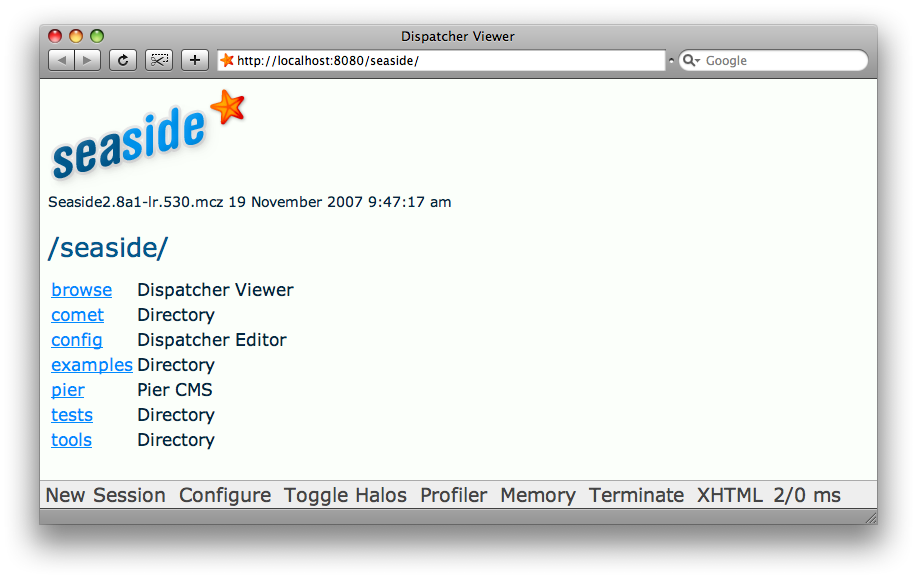
\includegraphics[width=\textwidth]{seasideStartup}
\caption{Iniciando Seaside}
\figlabel{seasideStartup}
\end{center}
\end{figure}

\dothis{Inicia el servidor Seaside y dirige un navegador web a \url{http://localhost:8080/seaside/}.}

\noindent
Deberías ver una página web como la de la \figref{seasideStartup}.

\noindent
\dothis{Navega a la página \lct{examples{\go}counter} page. (\figref{counter})}

\begin{figure}[htb]
\begin{center}
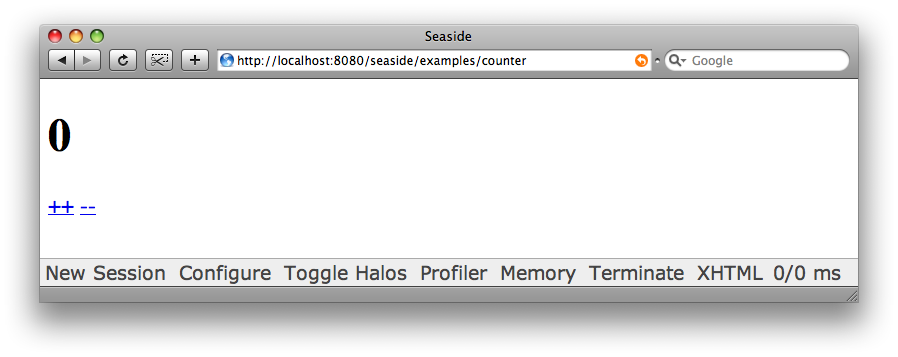
\includegraphics[width=0.8\textwidth]{counter}
\caption{El contador.}
\figlabel{counter}
\end{center}
\end{figure}

\noindent
Esta página es una pequeña aplicación Seaside: muestra un \subind{Seaside}{contador} que puede ser incrementado o decrementado haciendo click en los enlaces \link{++} y \link{--\,--}.

\noindent
\dothis{Juega con el contador haciendo click en estos enlaces.
Usa el botón ``atrás'' de tu navegador para volver a un estado previo y entonces haz cllick en \link{++} otra vez.
Fíjate cómo el contador se incrementa correctamente con respecto al estado mostrado en ese momento, en lugar del estado en que estaba cuando usaste el botón ``volver''.} 

Fíjate en la \subind{Seaside}{barra de herramientas} al final de la página web en la \figref{seasideStartup}.
Seaside soporta una noción de ``sesiones'' para realizar el seguimiento del estado de la aplicación para diferentes usuarios.
\button{New Session} comenzará una nueva sesión en la aplicación contador.
\button{Configure} permite configurar los ajustes de tu aplicación a través de una cómoda interfaz web.
(Para cerrar la vista \button{Configure}, pulsa en la \link{x} en la esquina superior derecha.)
\button{Toggle Halos} proporciona una forma de explorar el estado de la aplicación ejecutándose en el servidor Seaside.
\button{Profiler} y \button{Memory} proporcionan información detallada sobre el rendimiento de la aplicación en tiempo de ejecución.
\button{XHTML} puede usarse para validar la página web generada, pero sólo funciona cuando la página web es públicamente accesible en Internet porque usa el servicio de validación del W3C.
\index{Seaside!halos}

Las aplicaciones Seaside se construyen a partir de ``componentes'' conectables.
De hecho, los componentes son objetos normales de Smalltalk.
Lo único que tienen de especial es que deben ser instancias de clases que heredan de la clase \ct{WAComponent} del marco de trabajo Seaside.
Podemos explorar los componentes y sus clases desde la imagen \pharo o directamente desde la interfaz web usando los halos.

\begin{figure}[ht]
\begin{center}
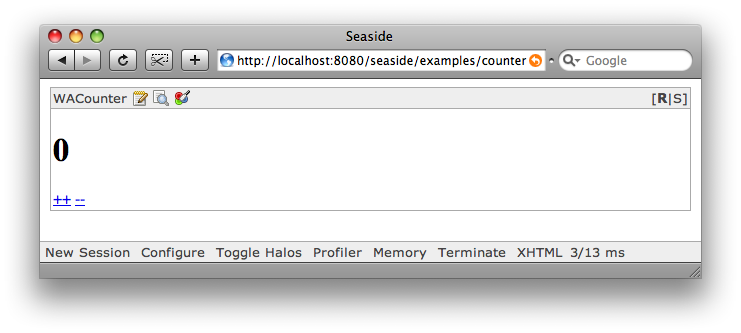
\includegraphics[width=\textwidth]{counterHalos}
\caption{Halos}
\figlabel{counterHalos}
\end{center}
\end{figure}

\dothis{Selecciona \button{Toggle Halos}. Deberías ver una página web como la de la \figref{counterHalos}.
En la esquina superior izquierda el texto \ct{WACounter} indica la clase del componente Seaside que implementa el comportamiento de esta página web.
Junto a este, hay tres iconos que puedes pulsar.
El primero, con el lápiz, activa el navegador de clases de Seaside sobre esta clase.
El segundo, con la lupa, abre un inspector de objetos sobre la instancia \ct{WACounter} actualmente activa.
El tercero, con los circulos de color, muestra la hoja de estilos \ind{CSS} para este componente.
En la esquina superior derecha, la \link{R} y \link{S} te permiten conmutar entre las vistas renderizadas y fuente de la página web.
Experimenta con todos estos enlaces.
Ten en cuenta que los vínculos \link{++} y \link{--} también están activos en la vista fuente.
Compara la vista fuente correctamente formateada que proporciona los Halos con la vista fuente sin formato ofrecida por tu navegador.}

El navegador de clases y el inspector de objetos de Seaside pueden ser muy útiles cuando el servidor está ejecutándose en otro ordenador, especialmente cuando el servidor no tiene pantalla o está en un lugar remoto.
Sin embargo, cuando desarrollas una aplicación Seaside por vez primera, el servidor estará ejecutándose localmente y es fácil usar las herramientas de desarrollo normales de \pharo en la imagen del servidor.

\begin{figure}[ht]
\begin{center}
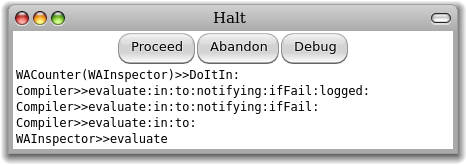
\includegraphics[width=0.7\textwidth]{haltingCounter}
\caption{Deteniendo el contador}
\figlabel{haltingCounter}
\end{center}
\end{figure}

\dothis{Usando el enlace del inspector de objetos en el navegador web, abrir un inspector sobre el objeto contador de Smalltalk subyacente y evaluar \ct{self halt}.
La página web detendrá la carga.
Ahora cambia a la imagen de Seaside.
Deberías ver una ventana de pre-depurador (\figref{haltingCounter}) mostrando un objeto \ct{WACounter} ejecutando un \ct{halt}.
Examina la ejecución en el depurador y entonces \button{Proceed}.
Vuelve al navegador web y fíjate en que la aplicación contador está ejecutándose otra vez.}

Los componentes de Seaside pueden instanciarse varias veces y en diferentes contextos.

\begin{figure}[ht]
\begin{center}
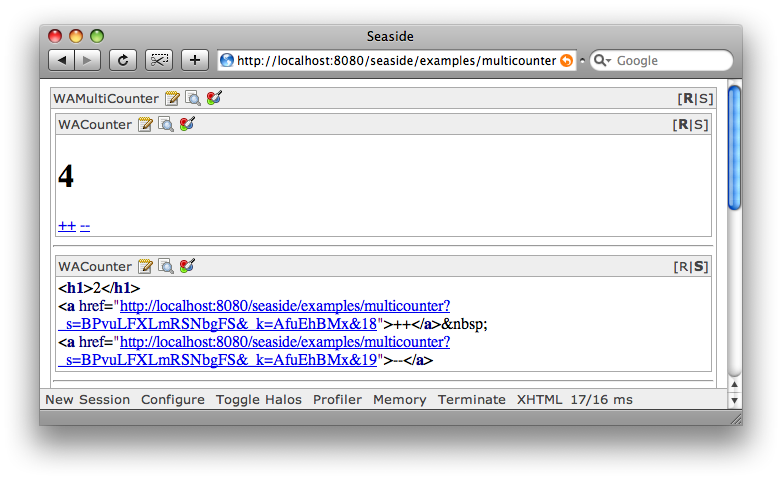
\includegraphics[width=\textwidth]{multiCounterHalos}
\caption{Subcomponentes independientes}
\figlabel{multiCounterHalos}
\end{center}
\end{figure}

\dothis{Dirige tu navegador web a \url{http://localhost:8080/seaside/examples/multicounter}.
Verás una aplicación formada por un número de instancias independientes del componente contador.
Incrementa y decrementa varios de los contadores.
Verifica que se comportan correctamente incluso si usas el botón ``atrás''.
Activa los halos para ver cómo la aplicación está formada por componentes anidados.
Usa el navegador de clases de Seaside para ver la implementación de  \ct{WAMultiCounter}.
Deberías ver tres métodos en el lado de clase (\ct{canBeRoot}, \ct{description} e \ct{initialize}) y tres en el lado de instancia (\ct{children}, \ct{initialize} y \ct{renderContentOn:}).
Observa que una aplicación es simplemente un componente dispuesto a ser la raíz de la jerarquía de componentes; esta predisposición se indica definiendo un método de clase \ct{canBeRoot} que responda \ct{true}.}
\index{Seaside!multi contador}

Puedes usar la interfaz web de Seaside para configurar, copiar o eliminar aplicaciones individuales (es decir, componentes del nivel raíz). Inteta realizar el siguiente cambio de configuración.

\dothis{Dirige tu navegador web a  \url{http://localhost:8080/seaside/config}.
Introduce el login y contraseña (\ct{admin} y \ct{seaside} por defecto).
Selecciona \link{Configure} junto a ``examples.''
Bajo la cabecera ``Add entry point'', introduce el nuevo nombre ``counter2'' para el tipo \emph{Application} y pulsa sobre \button{Add} (ver \figref{counter2}).
En la siguiente pantalla, cambia \emph{Root Component} a \clsind{WACounter}, entonces haz click en \button{Save} y \button{Close}.
Ahora tenemos un nuevo contador instalado en  \url{http://localhost:8080/seaside/examples/counter2}.
Usa la misma interfaz de configuración para eliminar este punto de entrada.
}
\index{Seaside!configuración}


\begin{figure}[ht]
\begin{center}
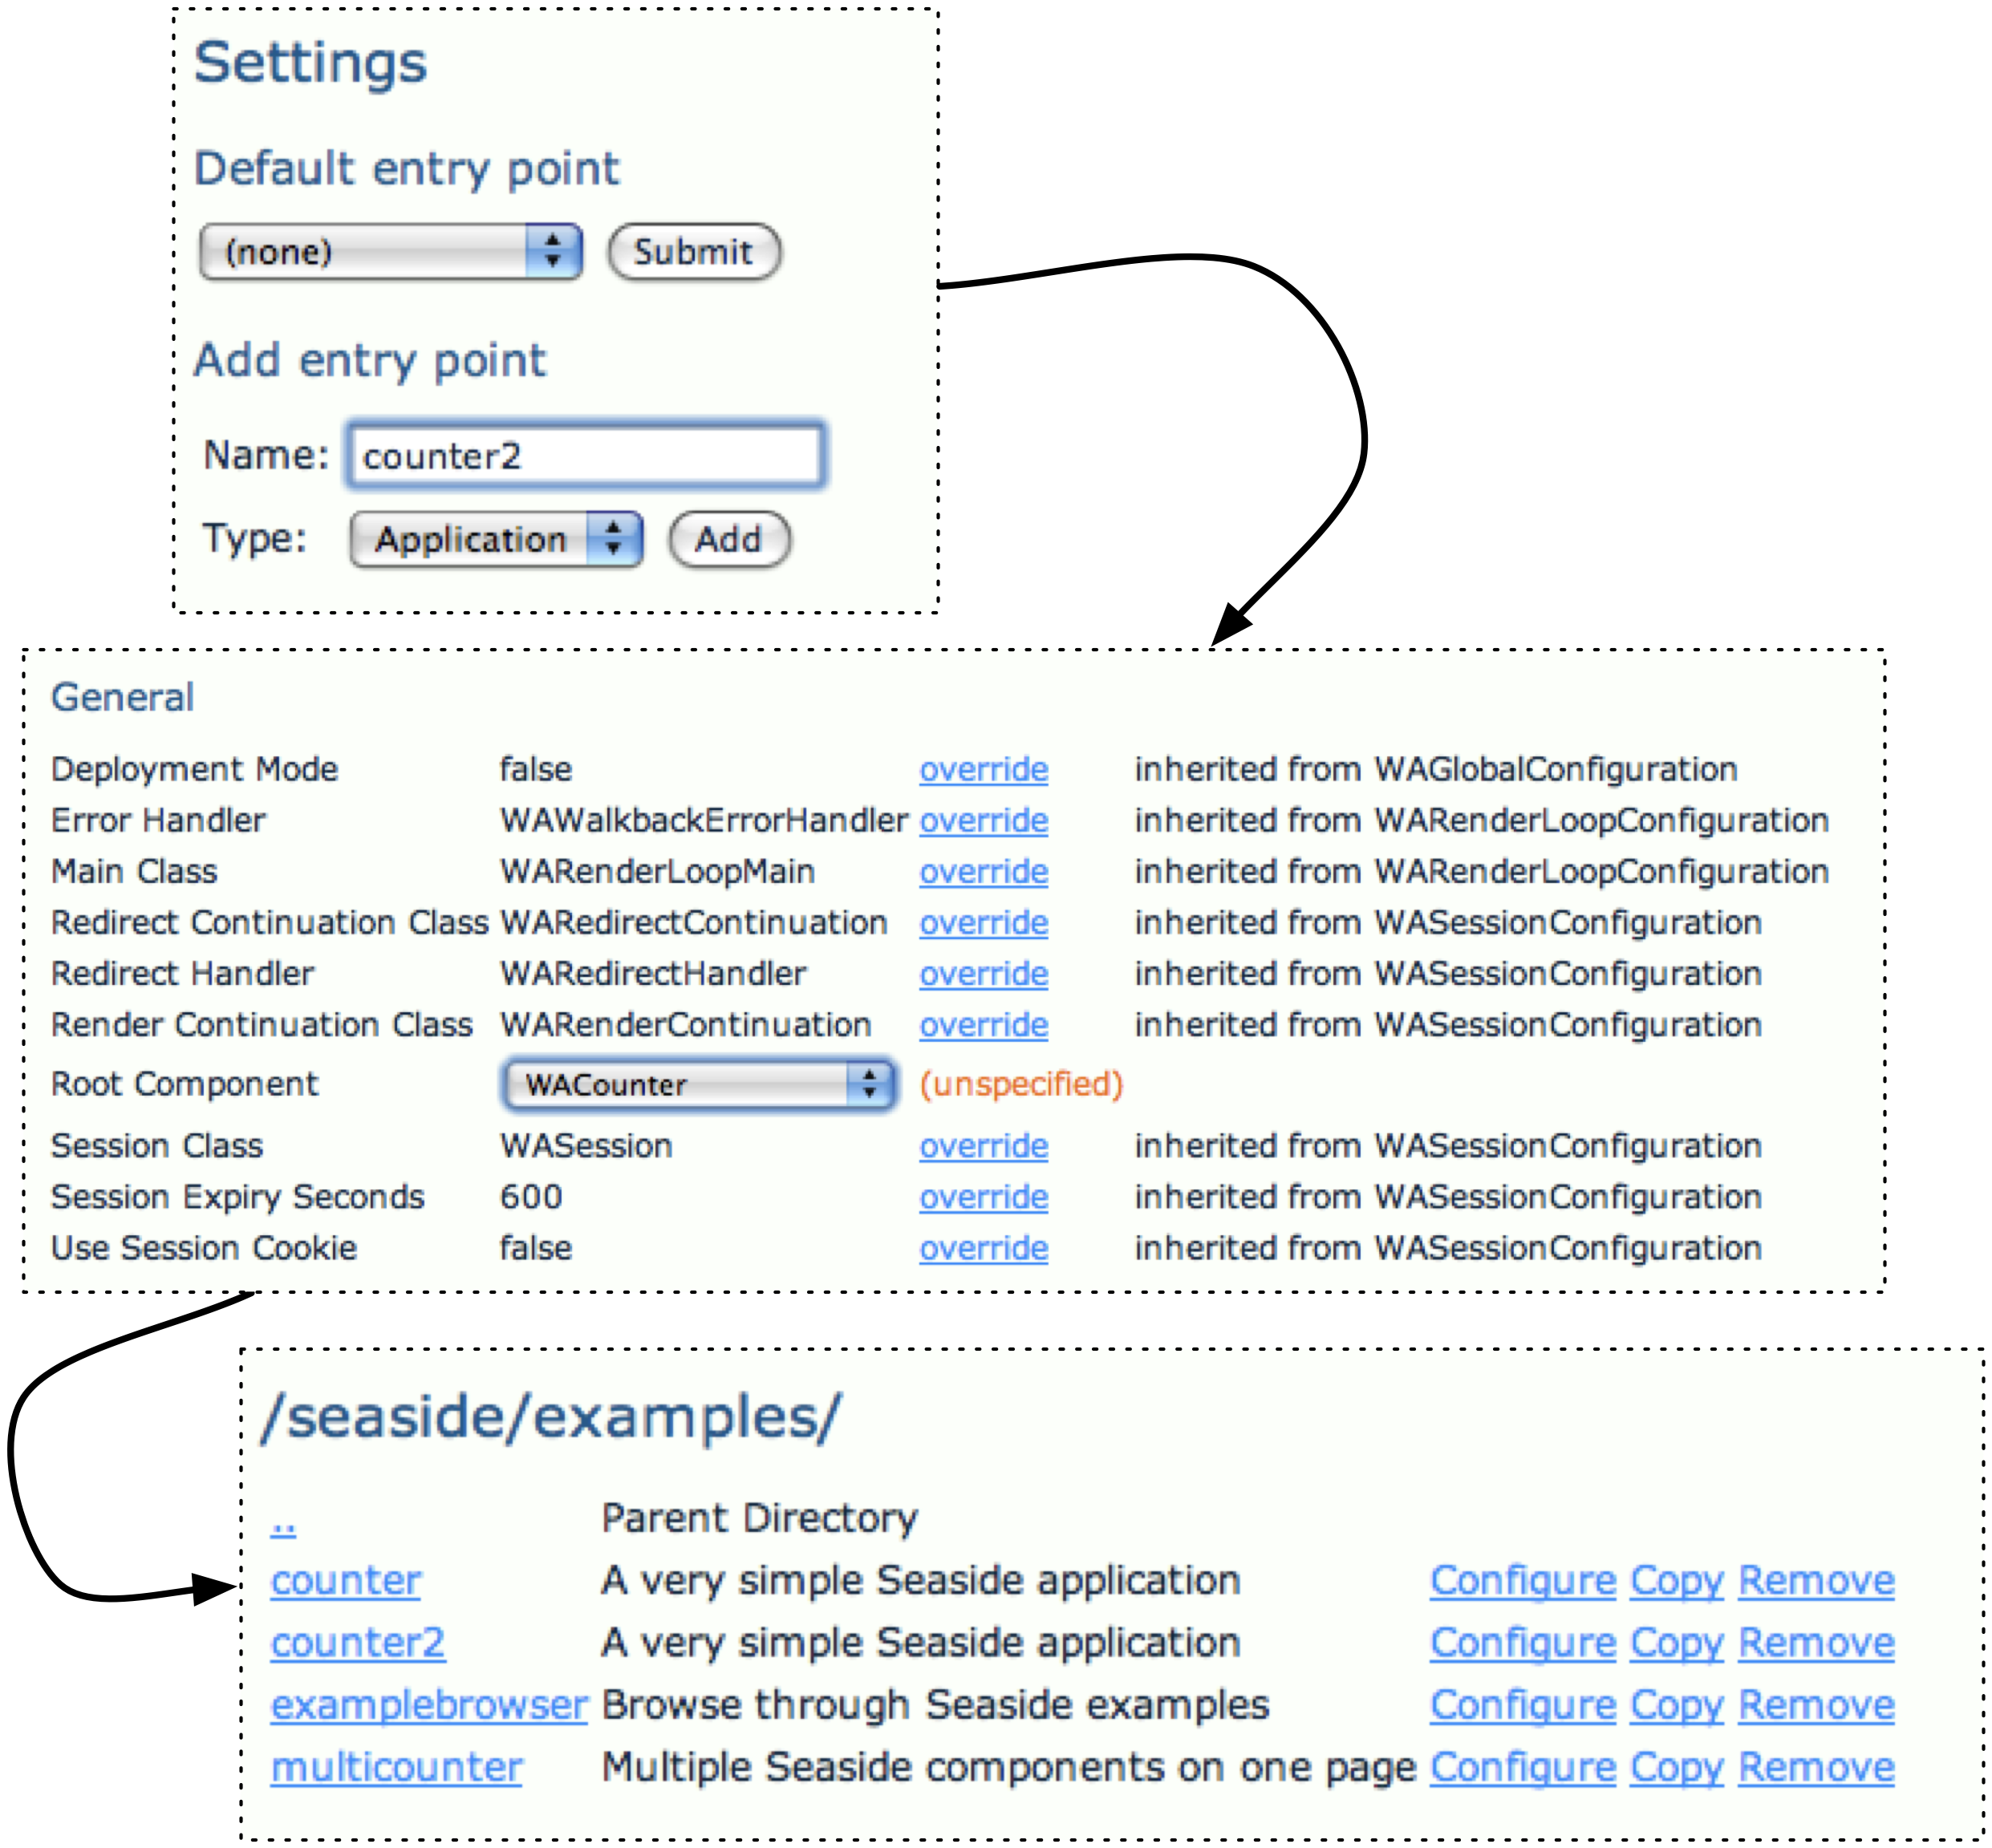
\includegraphics[width=\textwidth]{counter2}
\caption{Configuración de una nueva aplicación}
\figlabel{counter2}
\end{center}
\end{figure}

Seaside opera en dos modos: el modo \emph{desarrollo}, que es el que hemos visto hasta ahora, y el modo \emph{despliegue}, en el que la barra de herramientas no está disponible.
\index{Seaside!modo desarrollo}
\index{Seaside!modo despliegue}
Puedes poner Seaside en el modo despliegue usando la página de configuración (navega a la entrada para la aplicación y haz click en el enlace \link{Configure})
% \ab{How?  I couldn't find this}
o haciendo click en el botón \button{Configure} en la barra de herramientas.
En cualquier caso, se pone el modo despliegue a \emph{true}.
Observa que esto sólo afecta a las nuevas sesiones.
También puedes poner el modo globalmente evaluando
\clsind{WAGlobalConfiguration} \lct{setDeploymentMode}
o
\ct{WAGlobalConfiguration setDevelopmentMode}.
\index{Seaside!modo desarrollo}
\index{Seaside!modo despliegue}

La página web de configuración sólo es otra aplicación Seaside por lo que también puede ser controlada desde la página de configuración.
Si eliminas la aplicación ``config'', puedes recuperarla evaluando
\clsind{WADispatcherEditor} \ct{initialize}.

%=================================================================
\section{Componentes Seaside}
\seclabel{componentes}

%\ab{This section was too long\,---\,18 pages.  It also contained several self-references (``see section 1.3''). So I broke into smaller sections, by promoting some of the subsections and subsubsections.}

Como hemos mencionado en la sección anterior, las aplicaciones Seaside se construyen con \emph{\subind{Seaside}{componentes}}.
Vamos a estudiar detenidamente cómo funciona Seaside implementando el componente \emph{Hello World}.

Todo componente Seaside debe heredar directa o indirectamente de \clsind{WAComponent}, como muestra la figura \figref{WACounter}.

\dothis{Define una subclase de \ct{WAComponent} llamada \ct{WAHelloWorld}.}

Los componentes deben saber cómo representarse a sí mismos.
Normalmente esto se hace implementando el método \mthind{WAPresenter}{renderContentOn:}, que recibe como argumento una instancia de \clsind{WAHtmlCanvas}, que sabe cómo generar XHTML.
\index{Seaside!representación}

\dothis{Implementa el siguiente método y ponlo en un protocolo llamado \prot{rendering}:}

\needlines{2}
\begin{code}{}
WAHelloWorld>>>renderContentOn: html
	html text: 'hello world'
\end{code}

\noindent
Ahora debemos informar a Seaside de que este componente está dispuesto a ser una aplicación independiente.

\dothis{Implementa el siguiente método de clase de \ct{WAHelloWorld}.}

\begin{code}{}
WAHelloWorld class>>>canBeRoot
	^ true
\end{code}

\noindent
¡Estamos a punto de acabar!

\dothis{Dirige tu navegador web a \url{http://localhost:8080/seaside/config}, añade un nuevo punto de entrada llamado ``hello'' y pon como su componente raíz \ct{WAHelloWorld}.
Ahora dirige tu navegador a \url{http://localhost:8080/seaside/hello}.
!Ya está! Deberías ver una página web como la de la figura \figref{WAHelloWorld}.}


\begin{figure}[htb]
\begin{center}
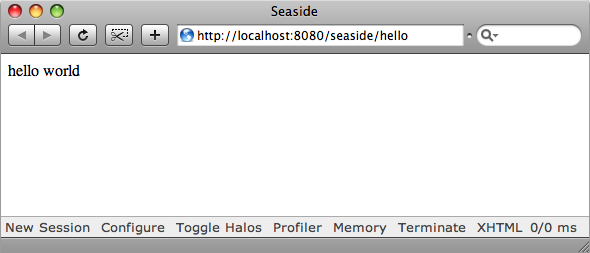
\includegraphics[width=\textwidth]{WAHelloWorld}
\caption{``Hello World'' en Seaside}
\figlabel{WAHelloWorld}
\end{center}
\end{figure}

%-----------------------------------------------------------------
\subsection{Marcha atrás de estado y la aplicación ``Counter''}
%{Simple and nested components}

La aplicación ``counter'' es sólo ligeramente más compleja que la aplicación ``hello world''.
\seclabel{backtracking}

\begin{figure}[ht]
\begin{center}
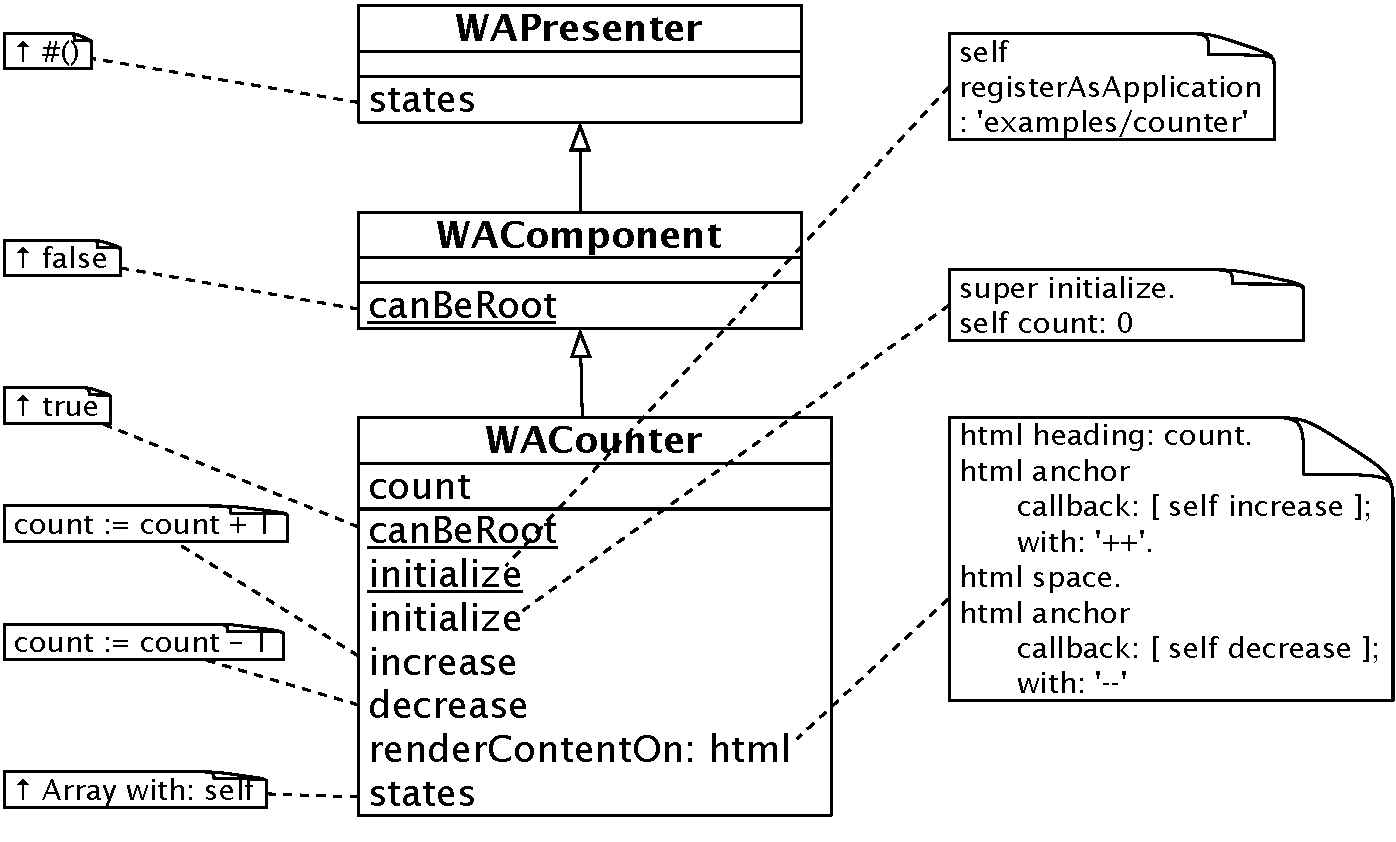
\includegraphics[width=\textwidth]{WACounter}
\caption{La clase \ct{WACounter}, que implementa la aplicación \emph{counter}. Los métodos con nombres subrayados son de clase; aquellos con nombres en texto normal son de instancia.}
\figlabel{WACounter}
\end{center}
\end{figure}

La clase \clsind{WACounter} es una aplicación independiente, con lo que la clase \ct{WACounter} debe responder \ct{true} al mensaje \mthind{WAComponent class}{canBeRoot}.
También debe registrarse como una aplicación; esto se hace en su método de clase \ct{initialize}, como muestra la figura \figref{WACounter}.
\ct{WACounter} define dos métodoso, \ct{increase} y \ct{decrease}, que serán disparados desde los vínculos \link{++} y \link{--\,--} de la página web.
También define una variable de instancia \ct{count} para registrar el estado del contador.
Sin embargo, también queremos que Seaside sincronice el contador con la página del navegador: cuando el usuario hace click en el botón ``atrás'' del navegador, queremos que Seaside ``retroceda'' el estado del objeto \ct{WACounter}.
Seaside incluye un mecaniso general de vuelta a atrás, pero cada aplicación tiene que decirle a Seaside qué partes de su estado tiene que seguir.

Un componente habilita la vuelta a atrás implementando el método \ct{states} en el lado de instancia:
% \ab{note that xspace messes up again, by inserting a space at the start of this line}
\ct{states} debería devolver un array que contenga todos los objetos a seguir.
En este caso, el objeto \ct{WACounter} se añade él mismo a la tabla de objetos que pueden retrocederse de Seaside Seaside devolviendo \ct{Array with: self}.

\paragraph{\emph{Advertencia.}}
Hay un punto sutil pero importante al que estar atento cuando se declaran objetos para retroceder.
Seaside sigue el estado haciendo una \emph{copia} de todos los objetos declarados en el array \ct{states}.
Hace esto usando un objeto \clsind{WASnapshot}; \ct{WASnapshot} es una subclase de \clsind{IdentityDictionary} que registra los objetos a seguir como claves y copias superficiales de su estado como valores.
\luq{\emph{shallow copy} como copia superficial}

Si el estado de una aplicación da marcha atrás a una instantánea particular, el estado de cada objeto que se añadió al diccionario de instantáneas se sobreescribe por la copia guardada en la instantánea. 
\luq{\emph{snapshot} traducido como instantánea}

El aspecto al que hay que estar atento es el siguiente:
En el caso de \ct{WACounter}, podrías pensar que el estado a seguir es un número\,---\,el valor de la variable de instancia \ct{count}.
Sin embargo, hacer que el método \ct{states} retorne \ct{Array with: count} no funcionará.  
Esto es así porque el objeto nombrado por \ct{count} es un entero y los enteros son inmutables.
Los métodos \ct{increase} y \ct{decrease} no cambian el estado del objeto \ct{0} a \ct{1} o el objeto \ct{3} a \ct{2}.
En cambio, \ct{count} nombra un entero diferente: 
cada vez que count se incrementa o decrementa, el objeto nombrado por \ct{count} es \emph{reemplazado} por otro.
Por esto es por lo que \ct{WACounter>>>states} debe retornar \ct{Array with: self}.
Cuando el estado de un objeto \mbox{\ct{WACounter}} es reemplazado por un estado previo, el \emph{valor} de cada una de las variables de instancia en el objeto es reemplazado por un valor previo; este reemplaza correctamente el valor actual de \ct{count} por un valor anterior. 
\index{Seaside!vuelta atrás del esstado}
\index{WAPresenter!states@\ct{states}}

\section{Generando XHTML}

El propósito de una aplicación web es crear o ``presentar'' páginas web.  Como mencionamos en \secref{components}, cada componente Seaside es responsable de presentarse a sí mismo.  
Así pues, vamos a comenzar nuestra exploración de la presentación viendo cómo el componente contador se presenta a sí mismo.

\subsection{Presentando el Contador}

La presentación del contador es relativamente directa; el código se muestra en la figura \figref{WACounter}.
El valor actual del contador se muestra como una cabecera XHTML, y las operaciones de incrementar y decrementar se implementan como anclas html (es decir, vínculos) con retrollamadas a bloques que enviarán \ct{increase} y \ct{decrease} al objeto contador.
\luq{\emph{callback} como retrollamada}

Echaremos un vistazo más de cerca al protocolo de presentación en un momento.
Pero antes de hacerlo, echemos un vistazo rápido al \subind{Seaside}{multi-contador}.

\subsection{De Contador a Multicontador}

\ct{WAMultiCounter} que se muestra en la figura \figref{WAMultiCounter} también es una aplicación independiente, con lo que sobreescribe \mthind{WAComponent class}{canBeRoot} para responder \ct{true}.
Además, es un componente \emph{compuesto}, con lo que Seaside requiere que declare sus hijos implementando un método \ct{children} que responda con un array con todos los componentes que contiene.
Se presenta a sí mismo presentando cada uno de sus subcomponentes, separados por una línea horizontal.
Además de los métodos de inicialización de instancia y estáticos, no hay nada más en el multicontador.

\begin{figure}[bht]
\begin{center}
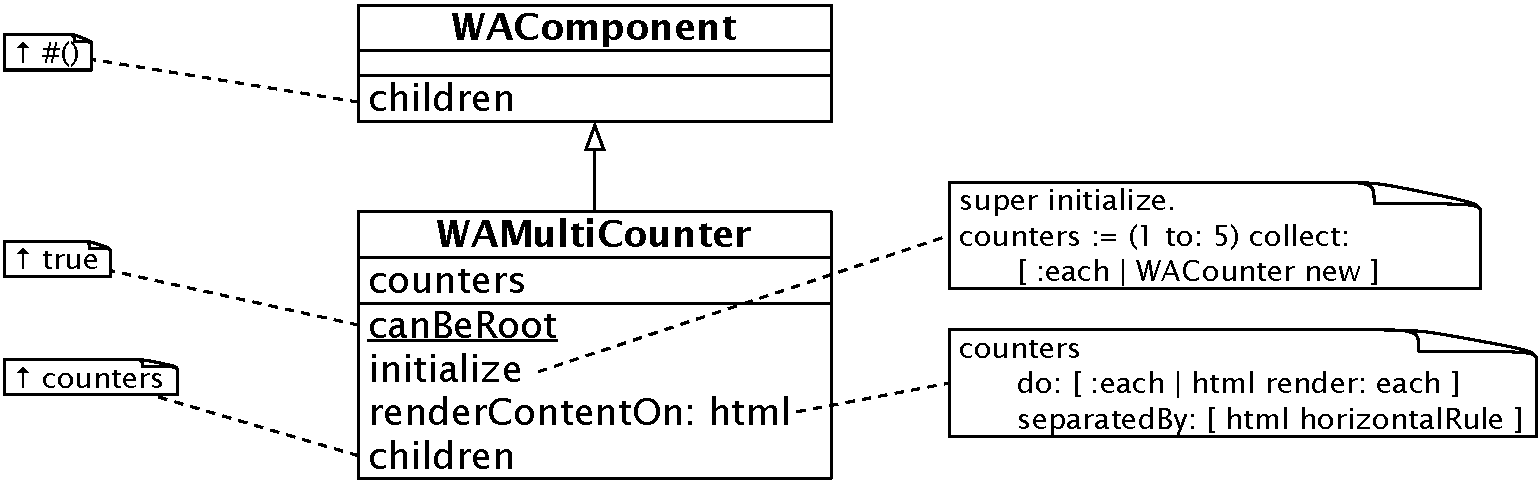
\includegraphics[width=\textwidth]{WAMultiCounter}
\caption{WAMultiCounter}
\figlabel{WAMultiCounter}
\end{center}
\end{figure}

%-----------------------------------------------------------------
\subsection{Más sobre la Presentación XHTML}

Como puedes ver en estos ejemplos, Seaside no usa plantillas para generar páginas web.
En su lugar, genera XHTML programadamente.
La idea básica es que cada componente Seaside debería sobreescribir el método \mthind{WAPresenter}{renderContentOn:}; este mensaje será enviado por el marco de trabajo a cada componente que necesita ser presentado.
Este mensaje \ct{renderContentOn:} tendrá un argumento que es un \seeindex{lienzo}{lienzo html} \emphind{lienzo html} sobre el que el componente debe presentarse a sí mismo. Por convenio, el parámetro del lienzo html se llama \ct{html}.

Un lienzo html es análogo al lienzo gráfico usado por Morphic (y la mayoría de otros marcos de trabajo de dibujo) para abstraerse de los detalles dependientes del dispositivo de dibujo.
 
Estos son algunos de los métodos de presentación más básicos:
\begin{code}{}
html text: 'hello world'.  "presenta una cada de texto plano"
html html: '&ndash;'.     "presenta un conjuro XHTML"
html render: 1.              "presenta cualquier objeto"
\end{code}

El mensaje \ct{render: anyObject} se puede enviar a un lienzo html para presentar \ct{anyObject}; se utiliza normalmente para presentar subcomponentes. A \lct{anyObject} se le enviará el mensaje \ct{renderContentOn:}
esto es lo que ocurre en el multi-contador (ver la \figref{WAMultiCounter}).

\subsection{Usando Pinceles}
\seclabel{brushes}

Un lienzo proporciona un número de \emphind{pinceles} que pueden usarse para presentar (\ie ``pintar) contenido en el lienzo.
Hay lienzos para cada tipo de elemento XHTML \,---\,párrafos, tablas, listas y demás.
Para ver el protocolo completo de lienzos y métodos de utilidad, deberías navegar por la clase \clsind{WACanvas} y sus subclases.
El argumento para \ct{renderContentOn:} es realmente una instancia de la subclase \clsind{WARenderCanvas}.

Ya hemos visto el siguiente pincel utilizado en los ejemplos contador y multi-contador:
\needlines{2}
\begin{code}{}
html horizontalRule.
\end{code}

\begin{figure}[ht]
\begin{center}
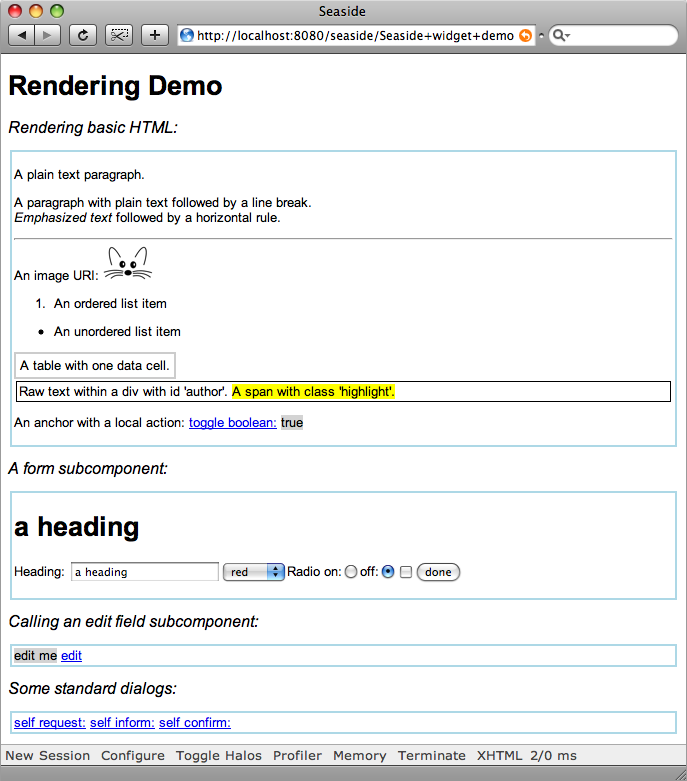
\includegraphics[width=\textwidth]{RenderingDemo}
\caption{RenderingDemo}
\figlabel{RenderingDemo}
\end{center}
\end{figure}

En la figura \figref{RenderingDemo} podemo ver la salida de muchos de los pinceles básicos ofrecidos por Seaside.\footnote{El código fuente para \mthref{renderdemo} está en el paquete \ct{PBE-SeasideDemo} en el proyecto \url{http://www.squeaksource.com/PharoByExample}.}
El componente raíz \ct{SeasideDemo} simplemente presenta sus subcomponentes, que son instancias de \ct{SeasideHtmlDemo}, \ct{SeasideFormDemo}, \ct{SeasideEditCallDemo} y \ct{SeasideDialogDemo}, como se muestra en \mthref{renderdemo}.

\needspace{7ex}
\begin{code}[renderdemo]{\lct{SeasideDemo>>renderContentOn:}}
SeasideDemo>>>renderContentOn: html
	html heading: 'Rendering Demo'.
	html heading
		level: 2;
		with: 'Rendering basic HTML: '.
	html div
		class: 'subcomponent';
		with: htmlDemo.
	"render the remaining components ..."
\end{code}

\noindent
Recuerda que un componente raíz debe siempre declarar sus hijos o Seaside rechazará presentarlos.
\begin{code}{}
SeasideDemo>>>children
	^ { htmlDemo . formDemo . editDemo . dialogDemo }
\end{code}

Ten en cuenta que hay dos formas distintas de instanciar el pincel \ct{heading}.
La primera forma es establecer el texto directamente enviando el mensaje \ct{heading:}.
La segunda forma es instanciar el pincel enviando \ct{heading} y entonces enviar una cascada de mensajes al pincel para establecer sus propiedades y presentarlo.

Muchos de los pinceles disponibles pueden usarse de estas dos formas.

\important{Si envías una \ind{cascada} de mensajes al pincel, incluyendo el mensaje \mthind{WABrush}{with:}, entonces \ct{with:} debería ser el mensaje \emph{final}.
\ct{with:} establece el contenido y presenta el resultado.}

En \mthref{renderdemo}, la primera cabecera está al nivel 1, ya que este es el valor por defecto.
Explícitamente ponemos el nivel de la segunda cabecera a 2.
El subcomponente es presentado como un \emph{div} XHTML con la clase \ind{CSS} ``subcomponent''.
(Más sobre CSS en \secref{css}.)
También ten en cuenta que es necesario que el argumento para el mensaje de palabra clave \ct{with:} no sea una cadena literal: puede ser otro componente, o incluso\,---\,como en el siguiente ejemplo\,---\,un bloque conteniendo más acciones de presentación.

El componente \ct{SeasideHtmlDemo} demuestra muchos de los pinceles más básicos.
La mayoría del código debería explicarse por sí solo.

\begin{code}{}
SeasideHtmlDemo>>>renderContentOn: html 
	self renderParagraphsOn: html.
	self renderListsAndTablesOn: html.
	self renderDivsAndSpansOn: html.
	self renderLinkWithCallbackOn: html
\end{code}

Es una práctica común dividir métodos de presentación largos en muchos métodos auxiliares, como hemos hecho aquí.

\important{No pongas todo tu código de presentación en un único método.
Divídelo en métodos auxiliares nombrados usando el patrón \ct{render*On:}.
Todos los métodos de presentación van en el protocolo \prot{rendering}.
No envíes \ct{renderContentOn:} desde tu propio código, usa \ct{render:} en su lugar.}

Mira el siguiente código.
El primer método auxiliar, \ct{SeasideHtmlDemo>>>renderParagraphsOn:}, muestra cómo generar párrafos XHTML, texto plano y enfatizado e imágenes.
Ten en cuenta que en Seaside los elementos sencillos son presentados especificando el texto que contienen directamente, mientras que los elementos complejos se especifican usando bloques.
Este es un convenio sencillo para ayudatte a estructurar tu código de presentación.

\begin{code}{}
SeasideHtmlDemo>>>renderParagraphsOn: html 
	html paragraph: 'Un parrafo con texto plano.'.
	html paragraph: [
		html
			text: 'Un parrafo con texto plano seguido por una nueva linea. ';
			break;
			emphasis: 'Texto con enfasis ';
			text: 'seguido por una linea horizontal.';
			horizontalRule;
			text: 'Una URI de imagen: '.
		html image
			url: self squeakImageUrl;
			width: '50']
\end{code}

El siguiente método auxiliar, \ct{SeasideHtmlDemo>>>renderListsAndTablesOn:}, muestra cómo generar listas y tablas.
Una tabla usa dos niveles de bloques para mostrar cada una de sus filas y las celdas dentro de las filas.

\begin{code}{}
SeasideHtmlDemo>>>renderListsAndTablesOn: html 
	html orderedList: [
		html listItem: 'Un elemento de una lista ordenada'].
	html unorderedList: [
		html listItem: 'Un elemento de una lista desordenada'].
	html table: [
		html tableRow: [
			html tableData: 'Una tabla con una celda de datos.']]
\end{code}

El siguiente ejemplo muestra cómo podemos especificar \emph{div}s y \emph{span}s con atributos CSS \emph{class} o \emph{id}.
Por supuesto, los mensajes \ct{class:} e \ct{id:} también pueden enviarse a los otros pinceles, no sólo a \emph{div}s y \emph{span}s.
El método \ct{SeasideDemoWidget>>>style} define cómo deberían ser mostrados estos elementos XHTML (ver \secref{css}).

\begin{code}{}
SeasideHtmlDemo>>>renderDivsAndSpansOn: html 
	html div
		id: 'author';
		with: [
			html text: 'Texto plano con un div con id ''author''. '.
			html span
				class: 'highlight';
				with: 'Un span con class ''highlight''.']
\end{code}

Finalmente vemos un sencillo ejemplo de un vínculo, creado asociando una sencilla \subind{Seaside}{retrollamada} con un ``ancla'' (\ie un vínculo).
Hacer click en el vínculo causará que el texto a continuación cambie entre ``true'' y ``false'' cambiando la variable de instancia \ct{toggleValue}.

\needlines{3}
\begin{code}{}
SeasideHtmlDemo>>>renderLinkWithCallbackOn: html 
	html paragraph: [
		html text: 'Un ancla con una accion local: '.
		html span with: [
			html anchor
				callback: [toggleValue := toggleValue not];
				with: 'cambia el booleano:'].
		html space.
		html span
			class: 'boolean';
			with: toggleValue ]
\end{code}

\important{Ten en cuenta que las acciones deberían aparecer sólo en retrollamadas.
¡El código ejecutado durante la presentación no debería cambiar el estado de la aplicación!}

%-----------------------------------------------------------------
\subsection{Formularios}

Los formularios se presentan igual que los otros ejemplos que ya hemos visto.
Este es el código para el componente \ct{SeasideFormDemo} de la figura \figref{RenderingDemo}.
\index{Seaside!formularios XHTML}

\begin{code}{}
SeasideFormDemo>>>renderContentOn: html
	| radioGroup |
	html heading: heading.
	html form: [
		html span: 'Cabecera: '.
		html textInput on: #heading of: self.
		html select
			list: self colors;
			on: #color of: self.
		radioGroup := html radioGroup.
		html text: 'Radio on:'.
		radioGroup radioButton
			selected: radioOn;
			callback: [radioOn := true].
		html text: 'off:'.
		radioGroup radioButton
			selected: radioOn not;
			callback: [radioOn := false].
		html checkbox on: #checked of: self.
		html submitButton
			text: 'hecho' ]
\end{code}{}

Puesto que un formulario es una entidad compleja, se presenta usando un bloque.
Ten en cuenta que todos los cambios de estado ocurren en las retrollamadas, no como parte de la presentación.

Hay una característica de Seaside utilizada aquí que merece una mención especial, que es el mensaje \mthind{WAAnchorTag}{on:of:}.
En el ejemplo, este mensaje se usa para asociar un campo de entrada de texto con la variable \ct{heading}.
Anclas y botones también soportan este mensaje.
El primer argumento es el nombre de una variable de instancia para la que se han definido métodos de acceso; el segundo argumento es el argumento al que esta variable de instancia pertenece.
Ambos métodos de acceso, observador (\ct{heading}) y modificador (\ct{heading:}) son comprendidos por el objeto con el convenio de nombre habitual.
En este caso de un campo de entrada de texto, esto nos ahorra el problema de tener que definir una retrollamada que actualice el campo además de tener que asociar los contenidos por defecto del campo de entrada html con el valor actual de la variable de instancia.
Usando \ct{on: #heading of: self}, la variable \ct{heading} se actualiza automáticamente cuando el usuario actualiza el campo de entrada de texto.

El mismo mensaje se usa dos veces más en este ejemplo, para causar que la selección de un color en el formulario html actualice la variable \ct{color}, y para asociar el resultado del checkbox con la variable \ct{checked}.
Muchos otros ejemplos pueden encontrarse en los tests funcionales de Seaside.
Echa un vistazo a la categoría \scat{Seaside-Tests-Functional}, o simplemente dirige tu navegador a \url{http://localhost:8080/seaside/tests/alltests}.
Selecciona \menu{WAInputTest} y haz click en el botón \button{Restart} para ver la mayoría de las características de los formularios.

No olvides que si activas \button{Toggle Halos}, puedes navegar directamente por el código fuente de los ejemplos usando el navegador de clases de Seaside.

%-----------------------------------------------------------------
\section{CSS: Hojas de estilo en cascada}
\seclabel{css}

%\ab{I think that it just needs a few paragraphs telling the reader the key ideas behind CSS, and the new terminology that the CSS folks introduce, before going in to the details of how you define their "thingies".  Now I have forgotten what they call their "thingies" --- I know that there are effectively paragraph styles (divs) and character styles (spans), but I've forgotten what they call them.  So, I think that the text needs to tell the reader, for each thingie, (1) the CSS concept behind the thingie, (2) what it looks like in a CSS style sheet , (3) what it looks like in html, and (4) how to do it in Seaside.   Maybe (3) can be omitted, because it's not needed to use Seaside.}
% \on{I think we do most of that already.}

Las hojas de estilo en cascada\footnote{\url{http://www.w3.org/Style/CSS/}}, o \ind{CSS} para abreviar, han surgido como una forma estándar de separar el estilo del contenido para las aplicaciones web.
Seaside se basa en CSS para evitar llenar tu código de presentación con consideraciones de diseño.

Puedes establecer la hoja de estilos CSS para tus componentes web definiendo el método \ct{style}, que debería devolver una cadena conteniendo las reglas CSS para ese componente.
Los estilos de todos los componentes mostrados en una página web se unen entre sí, con lo que cada componente puede tener su propio estilo.
Una mejor aproximación puede ser definir una clase abstracta para tu aplicación web que defina un estilo común para todas sus subclases.

En realidad, para las aplicaciones desplegadas, es más habitual definir las hojas de estilos como archivos externos.
De esta forma el aspecto del componente está completamente separado de su funcionalidad.
(Echa un vistazo a \clsind{WAFileLibrary}, que proporciona un modo de servir archivos estáticos sin la necesidad de un servidor independiente.)

Si ya estás familiarizado con CSS, esto es todo lo que necesitas saber.
En caso contrario, continúa leyendo una breve descripción de CSS.

En lugar de codificar directamente los atributos de presentación en los elementos de texto y párrafos de tus páginas web, con CSS definirás diferentes clases de elementos y colocarás todas las consideraciones de presentación en una hoja de estilos separada.
Las entidades de tipo párrafo se llaman \emph{div}s y las entidades de tipo texto son \emph{span}s. 
Entonces se definen nombres simbólicos, como ``highlight'' (ver ejemplo de abajo), para el texto resaltado y se especifica en la hoja de estilos cómo se va a presentar el texto resaltado.

Fundamentalmente una hoja de estilos CSS consiste en un conjunto de reglas que especifican cómo formatear los elementos XHTML dados.
Cada regla consta de dos partes.
Existe un \emph{selector} que especifica a qué elementos XHTML aplica la regla y una \emph{declaración} que define un número de atributos para esos elementos.

\begin{figure}[tb]
\begin{code}{}
SeasideDemoWidget>>>style
	^ '
body {
	font: 10pt Arial, Helvetica, sans-serif, Times New Roman;
}
h2 {
	font-size: 12pt;
	font-weight: normal;
	font-style: italic;
}
table { border-collapse: collapse; }
td {
	border: 2px solid #CCCCCC;
	padding: 4px;
}
#author {
	border: 1px solid black;
	padding: 2px;
	margin: 2px;
}
.subcomponent {
	border: 2px solid lightblue;
	padding: 2px;
	margin: 2px;
}
.highlight { background-color: yellow; }
.boolean { background-color: lightgrey; }
.field { background-color: lightgrey; }
'
\end{code}
\caption{Hoja de estilo común de \lct{SeasideDemoWidget}.
\figlabel{democss}}
\end{figure}

La \figref{democss} representa una hoja de estilo sencilla para la demo de presentación mostrada anteriormente en la \figref{RenderingDemo}.
La primera regla especifica una preferencia para la tipografía a utilizar por el \ct{body} de la página web.
Las siguientes reglas especifican propiedas de las cabeceras de segundo nivel (\ct{h2}), tablas (\ct{table}) y datos de las tablas (\ct{td}).

El resto de reglas tienen selectores que corresponden con los elementos XHTML que tengan los atributos ``class'' o``id''.
Los selectores CSS para los atributos clase comienzan con un ``\ct{.}'' y aquellos para los atributos id con ``\ct{#}''.
La principal diferencia entre los atributos clase e id es que muchos elementos pueden tenir la misma clase, pero sólo un elemento muy tener un id dado (\ie un \emph{identificador}). 
Así que, mientras un atributo clase, como \ct{highlight}, puede aparecer varias veces en cualquier página, un id debe identificar un elemento \emph{único} en la página, como un menú particular, la fecha de modificación o el autor.
Ten en cuanta que un elemento XHTML concreto puede tener varias clases, en cuyo caso todos los atributos de presentación se aplicarán en secuencia.

% This style sheet expects at most one element to specify the \emph{author} of the web page.

Las condiciones de los selectores pueden combinarse, con lo que el selector \ct{div.subcomponent} sólo se aplicará a aquellos elementos XHTML que sean un div \emph{y} tengan una atributo clave igual a ``subcomponent''.

También es posible especificar elementos anidados, aunque rara vez es necesario.
Por ejemplo, el selector ``\ct{p span}'' aplicará a un span dentro de un párrafo, pero no dentro de un div.

Existen muchos libros y sitios web que pueden ayudarte a aprender CSS.
Para una espectacular demostración del poder de CSS, te recomendamos que eches un vistazo al Jardín Zen CSS\footnote{\url{http://www.csszengarden.com/}}, que muestra cómo el mismo contenido puede presentarse de maneras radicalmente diferentes simplemente cambiando la hoja de estilos CSS.

%-----------------------------------------------------------------
\section{Gestión del control del flujo}

Seaside hace especialmente fácil diseñar aplicaciones web con un control de flujo no trivial.
Fundamentalmente existen dos mecanismos que puedes utilizar:

\begin{enumerate}
  \item Un componente puede \emph{llamar} a otro componente enviando \ct{visitante call: visitado}.
El visitante es reemplazado temporalmente por el visitado, hasta que el visitado devuelve el control enviando \ct{answer:}.
El visitante normalmente es \ct{self}, pero también podría ser cualquier otro componente visible actualmente.

  \item Un flujo de trabajo puede definirse como una \emphsubind{Seaside}{tarea}.
  Esta es un caso especial de componente que hereda de \clsind{WATask} (en lugar de \clsind{WAComponent}). \seclabel{tarea}
  En lugar de definir \ct{renderContentOn:}, no define ningún contenido, sino que define un método \ct{go} que envía una serie de mensajes \ct{call:} para activar varios subcomponentes.
\end{enumerate}
\index{Seaside!control de flujo}

%-----------------------------------------------------------------
\subsection{LLamada y respuesta}

Llamada y respuesta se usan para producir diálogos sencillos.

Hay un ejemplo trivial de \ct{call:} y \ct{answer:} en la demo de presentación de la \figref{RenderingDemo}.
El componente \ct{SeasideEditCallDemo} muestra un campo de texto y un vínculo \emph{edit}.
La retrollamada para el vínculo \emph{edit} llama a una nueva instancia de \ct{SeasideEditAnswerDemo} inicializada con el valor del campo de texto.
La retrollamada también actualiza este campo de texto con el resultado que se envía como respuesta.

(Subrayamos los mensajes \ct{call:} y \ct{answer:} enviados para llamar la atención sobre ellos.)

\begin{code}{}
SeasideEditCallDemo>>>renderContentOn: html 
	html span
		class: 'field';
		with: self text.
	html space.
	html anchor
		callback: [self text: (self !\underline{call:}! (SeasideEditAnswerDemo new text: self text))];
		with: 'edit'
\end{code}{}

Lo que resulta especialmente elegante es que el código no hace absolutamente ninguna referencia a la nueva página web que debe crearse.
En tiempo de ejecución, se crea una nueva página en la que el componente \ct{SeasideEditCallDemo} es reemplazado por un componente \ct{SeasideEditAnswerDemo}; el componente padre y el resto de componentes no se ven modificados.

\important{\mthind{WAComponent}{call:} y \mthind{WAComponent}{answer:} nunca deben usarse durante la presentación.
Pueden ser enviados de forma segura desde una \subind{Seaside}{retrollamada} o desde el método \mthind{WATask}{go} de una tarea.}

El componente \ct{SeasideEditAnswerDemo} también es extraordinariamente sencillo.
Simplemente presenta un formulario con un campo de texto.
El botón de envío está vinculado con una retrollamada que responderá el valor final del campo de texto.

\begin{code}{}
SeasideEditAnswerDemo>>>renderContentOn: html
	html form: [
		html textInput
			on: #text of: self.
		html submitButton
			callback: [ self !\underline{answer:}! self text ];
			text: 'ok'.
		]
\end{code}{}

Eso es todo.

Seaside se ocupa del control del flujo y de la correcta presentación de todos los componentes.
Curiosamente, el botón ``volver'' del navegador también funcionará correctamente (aunque los efectos colaterales no se deshacen a no ser que añadamos algunos pasos adicionales).

%-----------------------------------------------------------------
\subsection{Métodos de utilidad}
\luq{convenience methods como métodos de utilidad?}

Puesto que ciertos diálogos llamada--respuesta son muy comunes, Seaside proporciona algunos métodos de utilidad para ahorrarte el problema de escribir componentes como \ct{SeasideEditAnswerDemo}.
Los diálogos generados se muestran en la \figref{dialogs}.
Podemos ver los métodos de utilidad empleados en \ct{SeasideDialogDemo>>>renderContentOn:}
\index{Seaside!métodos de utilidad}

\begin{figure}[b]
\begin{center}
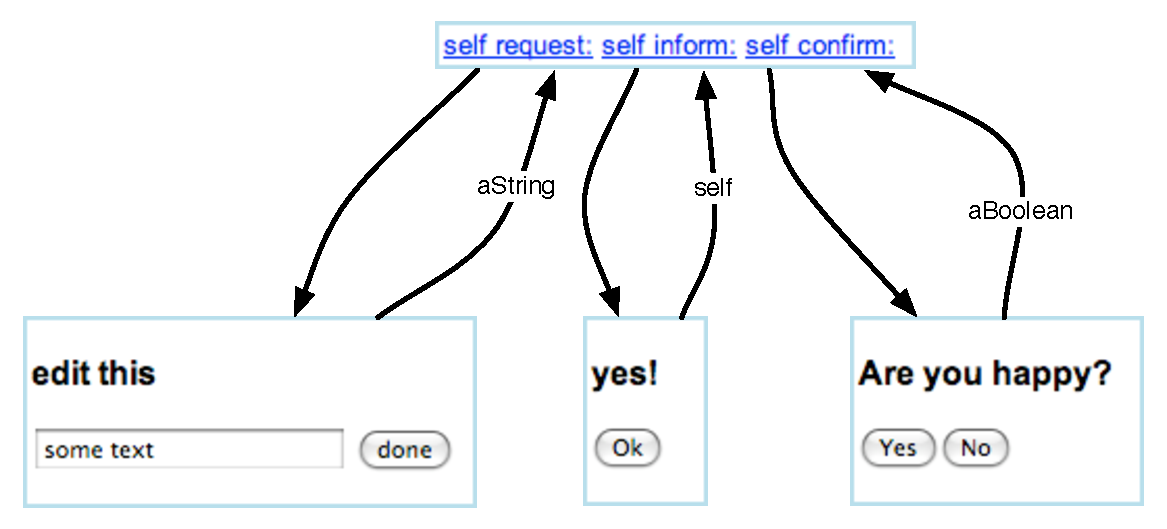
\includegraphics[width=\textwidth]{dialogs}
\caption{Algunos diálogos estándar}
\figlabel{dialogs}
\end{center}
\end{figure}

El mensaje \mthind{WAComponent}{request:} realiza una llamada a un componente que te permitirá editar un campo de texto.
El componente responde con la cadena editada.
También pueden especificarse opcionalmente una etiqueta y un valor por defecto.

\needlines{3}
\begin{code}{}
SeasideDialogDemo>>>renderContentOn: html
	html anchor
		callback: [ self request: 'edit this' label: 'done' default: 'some text' ];
		with: 'self request:'.
...
\end{code}

El mensaje \mthind{WAComponent}{inform:} llama a un componente que simplemente muestra el mensaje del argumento y espera a que el usuario pulse en ``ok''.
El componente llamada simplemente retorna \ct{self}.

\begin{code}{}
...
	html space.
	html anchor
		callback: [ self inform: 'yesBANG' ];
		with: 'self inform:'.
...
\end{code}

El mensaje \mthind{WAComponent}{confirm:} realiza una pregunta y espera a que el usuario seleccione ``Yes'' o ``No''.
El componente responde con un booleano, que puede utilizarse para realizar otras acciones.

\begin{code}{}
...
	html space.
	html anchor
		callback: [
			(self confirm: 'Are you happy?')
				ifTrue: [ self inform: ':-)' ]
				ifFalse: [ self inform: ':-(' ]
			];
		with: 'self confirm:'.
\end{code}

Algunos otros métodos de utilidad, como \mthind{WAComponent}{chooseFrom:caption:}, se definen en el protocolo \prot{convenience} de \clsind{WAComponent}.

%-----------------------------------------------------------------
\subsection{Tareas}

Una \subind{Seaside}{tarea} es un componente que hereda de \clsind{WATask}.
No presenta nada por sí misma, sino que simplemente llama a otros componentes en un control de flujo definido implementando el método \mthind{WATask}{go}.

\clsind{WAConvenienceTest} es un ejemplo sencillo de una tarea definida en la categoría \scat{Seaside-Tests-Functional}.
Para ver sus efectos, simplemente dirige tu navegador a \url{http://localhost:8080/seaside/tests/alltests}, selecciona \menu{WAConvenienceTest} y haz click en \button{Restart}.

\begin{code}{}
WAConvenienceTest>>>go
	[ self chooseCheese.
	  self confirmCheese ] whileFalse.
	self informCheese
\end{code}

Esta tarea llamada a su vez a tres componentes.
El primero, generado por el método de utilidad \mthind{WAComponent}{chooseFrom: caption:}, es un \clsind{WAChoiceDialog} que pide al usuario que escoja un queso.

\begin{code}{}
WAConvenienceTest>>>chooseCheese
	cheese := self
		chooseFrom: #('Greyerzer' 'Tilsiter' 'Sbrinz')
		caption: 'What''s your favorite Cheese?'.
	cheese isNil ifTrue: [ self chooseCheese ]
\end{code}

% \alex{Is there a situation where cheese may be nil? Maybe if a browser authorizes an empty selection...}

El segundo es un \clsind{WAYesOrNoDialog} para confirmar la elección (generado por el método de utilidad \mthind{WAComponent}{confirm:}).

\begin{code}{}
WAConvenienceTest>>>confirmCheese
	^self confirm: 'Is ', cheese,  ' your favorite cheese?'
\end{code}

Finalmente se llama a un \clsind{WAFormDialog} (por medio del método de utilidad \mthind{WAComponent}{inform:}).

\begin{code}{}
WAConvenienceTest>>>informCheese
	self inform: 'Your favorite cheese is ', cheese, '.'
\end{code}

Los diálogos generados se muestran en la \figref{chooseCheese}.

\begin{figure}[ht]
\begin{center}
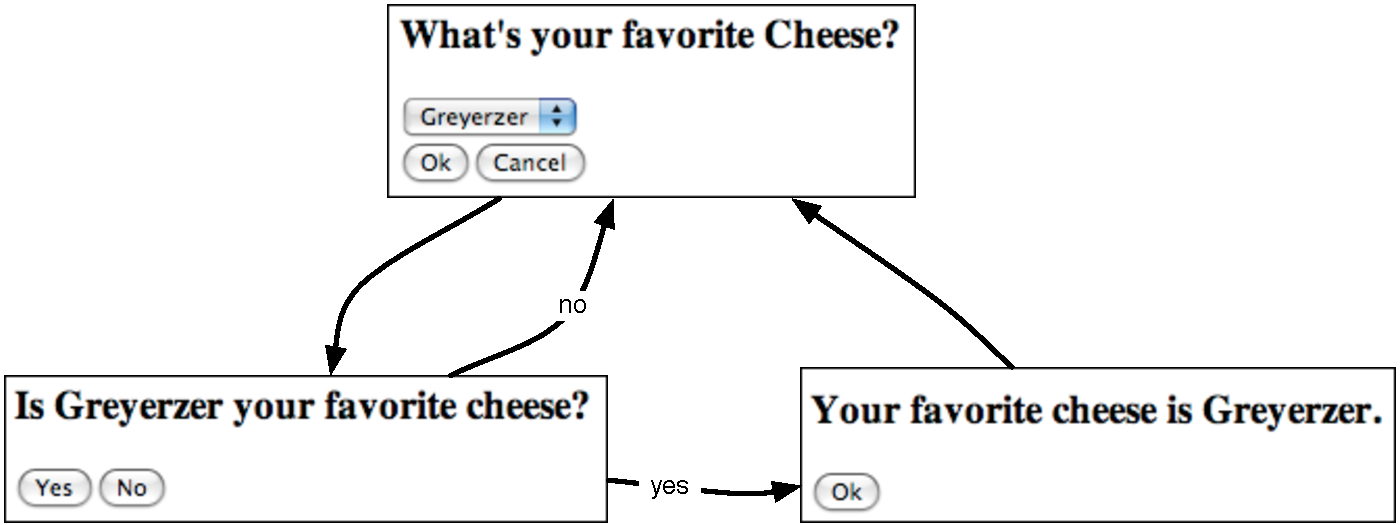
\includegraphics[width=\textwidth]{chooseCheese}
\caption{Una tarea sencilla}
\figlabel{chooseCheese}
\end{center}
\end{figure}

%-----------------------------------------------------------------
\subsection{Transacciones}

Como vimos en la \secref{backtracking}, Seaside puede realizar un seguimiento de la correspondencia entre el estado de los componentes y las páginas web individuales por medio de componentes que registran sus estados para la vuelta atrás:
todo lo que un componente necesita es implementar el método \ct{states} para devolver un array con todos los objetos cuyo estado debe seguirse.

Sin embargo, algunas veces, no queremos volver atrás el estado: en su lugar queremos \emph{evitar} que el usuario accidentalmente deshaga los efectos que deberían ser permanentes.
A esto nos referimos frecuentemente como ``el problema del carrito de la compra''.
Una vez que has validado tu carrito de la compra y pagado por los elementos que has comprado, no debería ser posible volver ``atrás'' con el navegador y añadir más elementos al carrito.

Seaside te permite evitar esto definiendo una tarea en la que ciertas acciones están agrupadas como \emph{transacciones}.
Puedes volver atrás dentro de una transacción, pero una vez que una transacción está completa, ya no puedes deshacerla.
Las páginas correspondientes están \emph{invalidadas} y cualquier intento de volver a ellas causará que Seaside genere un aviso y redirija al usuario a la página válida más reciente.

\begin{figure}[ht]
\begin{center}
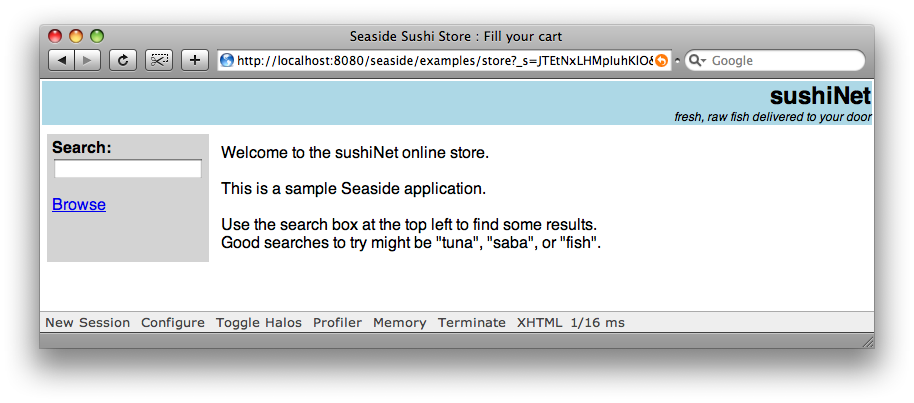
\includegraphics[width=\textwidth]{sushiStore}
\caption{La tienda de Sushi}
\figlabel{sushiStore}
\end{center}
\end{figure}

La aplicación de Seaside \emphsubind{Seaside}{Sushi Store} es una aplicación de ejemplo que ilustra muchas de las características de Seaside, incluyendo las transacciones.
La aplicación está incluída con tu instalación de Seaside, así que puedes probarla dirigiendo tu navegador a
\url{http://localhost:8080/seaside/examples/store}.\footnote{Si no puedes encontrarla en tu imagen, existe una versión de la tienda de sushi disponible en SqueakSource en \url{http://www.squeaksource.com/SeasideExamples/}.}

La tienda de sushi soporta el siguiente flujo:
\begin{enumerate}[itemsep=0pt]
  \item Visita la tienda.
  \item Navega o busca sushi.
  \item Añade sushi a tu carrito de la compra.
  \item Lanza el pedido.
  \item Verifica tu pedido.
  \item Introduce la dirección de entrega.
  \item Verifica la dirección de entrega.
  \item Introduce la información del pago.
  \item ¡Tu pescado está en camino!
\end{enumerate}

Si activas los \subind{Seaside}{halos}, verás que el componente de primer nivel de la tienda de sushi es una instancia de \clsind{WAStore}.
No hace nada, salvo presentar la barra de título y entonces presenta \ct{task}, una instancia de  \clsind{WAStoreTask}.

\begin{code}{}
WAStore>>>renderContentOn: html
	"... render the title bar ..."
	html div id: 'body'; with: task
\end{code}

\clsind{WAStoreTask} captura la secuencia de este flujo. En un par de puntos es crítico que el usuario no sea capaz de volver atrás y cambiar la información enviada.

\dothis{\,``Compra'' algo de sushi y entonces usa el botón ``atrás'' para intentar añadir más sushi al carrito.
Obttendrás el mensaje ``That page has expired.''}

Seaside permite al programador declarar que cierta parte de un flujo de trabajo actúa como una transacción: una vez que la transacción se completa, el usuario no puede volver atrás y deshacerla.
Declaras esto enviando \mthind{WAComponent}{isolate:} a una tarea con el bloque transaccional como su argumento.
Podemos ver esto en el flujo de trabajo de la tienda de sushi a continuación:

\begin{code}{}
WAStoreTask>>>go
	| shipping billing creditCard |
	cart := WAStoreCart new.
	self isolate:
		[[self fillCart.
		self confirmContentsOfCart]
			whileFalse].

	self isolate:
		[shipping := self getShippingAddress.
		billing := (self useAsBillingAddress: shipping)
					ifFalse: [self getBillingAddress]
					ifTrue: [shipping].
		creditCard := self getPaymentInfo.
		self shipTo: shipping billTo: billing payWith: creditCard].

	self displayConfirmation.
\end{code}

Aquí vemos bastante claramente que existen dos transacciones.
La primera rellena el carrito y cierra la fase de compra.
(Los métodos auxiliares \ct{fillCart} \etc se ocupan de instanciar y llamar a los componentes adecuados.)
Una vez que has confirmado los contenidos del carrito no puedes volver atrás sin iniciar una nueva sesión.
La segunda transacción cumplimenta los datos de envío y pago.
Puedes navegar atrás y adelante dentro de la segunda transacción hasta que confirmas el pago.
Sin emgargo, una vez que ambas transacciones estás completas, cualquier intento de navegar atrás fallará.

Las transacciones también pueden anidarse.
Una demostración sencilla de estos se encuentra en la clase \clsind{WANestedTransaction}.
El primer \ct{isolate:} recibe como argumento un bloque que contiene otro \ct{isolate:} anidado.

\begin{code}{}
WANestedTransaction>>>go
	self inform: 'Before parent txn'.
	self isolate:
			[self inform: 'Inside parent txn'.
			self isolate: [self inform: 'Inside child txn'].
			self inform: 'Outside child txn'].
	self inform: 'Outside parent txn'
\end{code}

\dothis{Ve a \url{http://localhost:8080/seaside/tests/alltests}, selecciona \menu{WATransactionTest} y pulsa en \button{Restart}.
Prueba a navegar atrás y adelante dentro de las transacciones padre e hija pulsando el botón \button{atrás} y después en \button{ok}.
Observa que tan pronto como una transacción se completa, ya no puedes volver atrás dentro de la transacción sin generar un error al pulsar \button{ok}.}

%=================================================================
\section{A complete tutorial example}

% ON: Should take about two hours

Let's see how we can build a complete Seaside application from scratch.\footnote{The exercise should take at most a couple of hours. If you prefer to just look at the completed source code, you can grab it from the SqueakSource project \url{http://www.squeaksource.com/PharoByExample}.
The package to load is \scat{PBE-SeasideRPN}. The tutorial that follows uses slightly different class names so that you can compare your implementation with ours.}
We will build a RPN (Reverse Polish Notation) calculator as a Seaside application that uses a simple stack machine as its underlying model.
Furthermore, the Seaside interface will let us toggle between two displays\,---\,one which just shows us the current value on top of the stack, and the other which shows us the complete state of the stack.
The calculator with the two display options is shown in \figref{stackMachine}.

\begin{figure}[ht]
\begin{center}
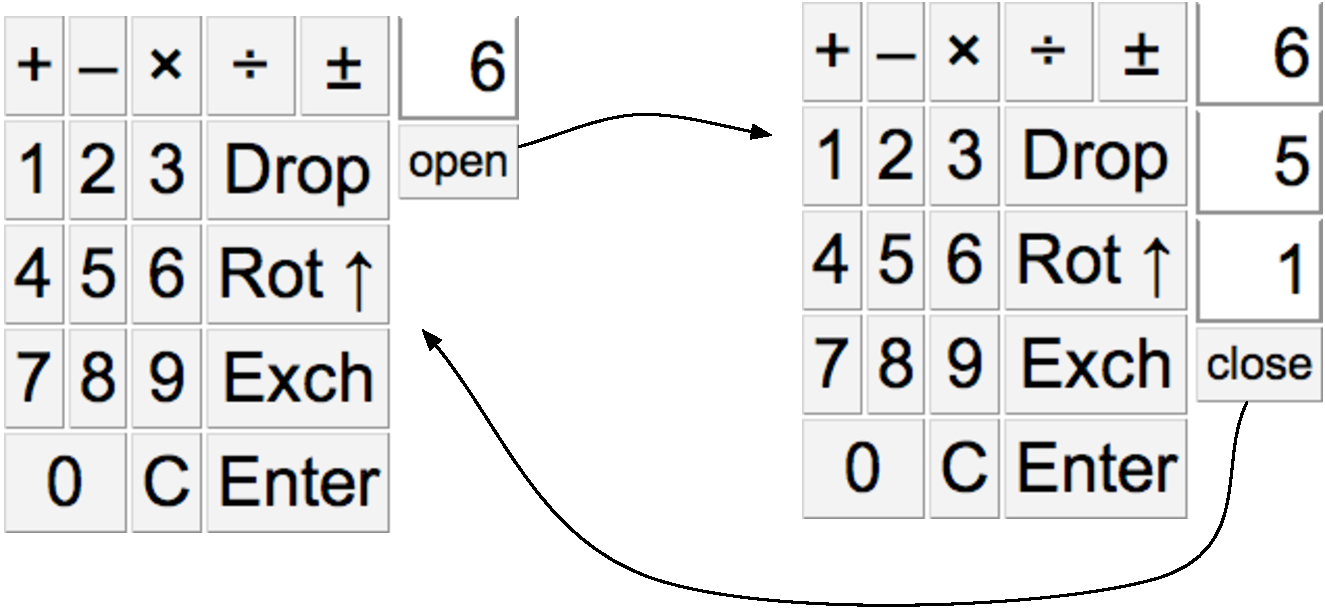
\includegraphics[width=\textwidth]{stackMachine}
\caption{RPN calculator and its stack machine}
\figlabel{stackMachine}
\end{center}
\end{figure}

We begin by implementing the stack machine and its tests.

\dothis{Define a new class called \ct{MyStackMachine} with an instance variable \ct{contents} initialized to a new \ct{OrderedCollection}.}

\begin{code}{}
MyStackMachine>>>initialize
	super initialize.
	contents := OrderedCollection new.
\end{code}

The stack machine should provide operations to \ct{push:} and \ct{pop} values, view the \ct{top} of the stack, and perform various arithmetic operations to add, subtract, multiply and divide the top values on the stack.

\dothis{Write some tests for the stack operations and then implement these operations.
Here is a sample test:}

\needlines{4}
\begin{code}{}
MyStackMachineTest>>>testDiv
	stack
		push: 3;
		push: 4;
		div.
	self assert: stack size = 1.
	self assert: stack top = (4/3).
\end{code}

You might consider using some helper methods for the arithmetic operations to check that there are two numbers on the stack before doing anything, and raising an error if this precondition is not fulfilled.\footnote{It's a good idea to use \ct{Object>>>assert:} to specify the preconditions for an operation.
This method will raise an \ct{AssertionFailure} if the user tries to use the stack machine in an invalid state.}
If you do this, most  of your methods will just be one or two lines long.

You might also consider implementing \ct{MyStackMachine>>>printOn:} to make it easier to debug your stack machine implementation with the help of an object inspector.
(Hint: just delegate printing to the \ct{contents} variable.)
\index{Object!printOn:@\ct{printOn:}}

\dothis{Complete the \ct{MyStackMachine} by writing operations \ct{dup} (push a duplicate of the top value onto the stack), \ct{exch} (exchange the top two values), and \ct{rotUp} (rotate the entire stack contents up\,---\,the top value will move to the bottom).}

Now we have a simple stack machine implementation.
We can start to implement the Seaside RPN Calculator.

We will make use of 5 classes:
\begin{itemize}
  \item \ct{MyRPNWidget}\,---\,this should be an abstract class that defines the common CSS style sheet for the application, and other common behavior for the components of the RPN calculator.
  It is a subclass of \ct{WAComponent} and the direct superclass of the following four classes. 
  
    \item \ct{MyCalculator}\,---\,this is the root component.
  It should register the application (on the class side), it should instantiate and render its subcomponents, and it should register any state for backtracking.
  \item \ct{MyKeypad}\,---\,this displays the keys that we use to interact with the calculator.
  \item \ct{MyDisplay}\,---\,this component displays the top of the stack and provides a button to call another component to display the detailed view.
  \item \ct{MyDisplayStack}\,---\,this component shows the detailed view of the stack and provides a button to answer back.
  It is a subclass of \lct{MyDisplay}.
\end{itemize}

\dothis{Define \ct{MyRPNWidget} in the category \ct{MyCalculator}.
Define the common \ct{style} for the application.}

Here is a minimal CSS for the application.
You can make it more fancy if you like.
\begin{code}{}
MyRPNWidget>>>style
	^ 'table.keypad { float: left; }
td.key {
	border: 1px solid grey;
	background: lightgrey;
	padding: 4px;
	text-align: center;
}
table.stack { float: left; }
td.stackcell {
	border: 2px solid white;
	border-left-color: grey;
	border-right-color: grey;
	border-bottom-color: grey;
	padding: 4px;
	text-align: right;
}
td.small { font-size: 8pt; }'
\end{code}

\dothis{Define \ct{MyCalculator} to be a root component and register itself as an application (\ie implement \ct{canBeRoot} and \ct{initialize} on the class side).
Implement \ct{MyCalculator>>>renderContentOn:} to render something trivial (such as its name), and verify that the application runs in a browser.
}

\ct{MyCalculator} is responsible for instantiating \ct{MyStackMachine}, \ct{MyKeypad} and \ct{MyDisplay}.

\dothis{
Define \ct{MyKeypad} and \ct{MyDisplay} as subclasses of \lct{MyRPNWidget}.
All three components will need access to a common instance of the stack machine, so define the instance variable \ct{stackMachine} and an initialization method \ct{setMyStackMachine:} in the common parent, \ct{MyRPNWidget}.
Add instance variables \ct{keypad} and \ct{display} to \ct{MyCalculator} and initialize them in \ct{MyCalculator>>>initialize}.
(Don't forget to send \lct{super initialize}!)}

\dothis{
Pass the shared instance of the stack machine to the keypad and the display in the same initialize method.
Implement \ct{MyCalculator>>>renderContentOn:} to simply render in turn the keypad and the display.
To correctly display the subcomponents, you must implement \ct{MyCalculator>>>children} to return an array with the keypad and the display.
Implement placeholder rendering methods for the keypad and the display and verify that the calculator now displays its two subcomponents.
}

%\ab{Too long!}

Now we will change the implementation of the display to show the top value of the stack.

\dothis{
Use a table with class ``keypad'' containing a row with a single table data cell with class ``stackcell''.
Change the rendering method of the keypad to ensure that the number 0 is pushed on the stack in case it is empty.
(Define and use \ct{MyKeypad>>>ensureMyStackMachineNotEmpty}.)
Also make it display an empty table with class ``keypad''.
Now the calculator should display a single cell containing the value 0.
If you toggle the halos, you should see something like this:
}

\begin{figure}[ht]
\begin{center}
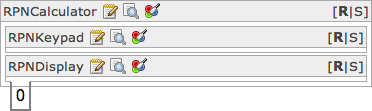
\includegraphics[width=0.8\textwidth]{firstStackDisplay}
\caption{Displaying the top of the stack}
\figlabel{firstStackDisplay}
\end{center}
\end{figure}

Now let's implement an interface to interact with the stack.

\dothis{
First define the following helper methods, which will make it easier to script the interface:
}

\needlines{3}
\begin{code}{}
MyKeypad>>>renderStackButton: text callback: aBlock colSpan: anInteger on: html 
	html tableData
		class: 'key';
		colSpan: anInteger;
		with: 
				[html anchor
					callback: aBlock;
					with: [html html: text]]
\end{code}


\begin{code}{}
MyKeypad>>>renderStackButton: text callback: aBlock on: html 
	self 
		renderStackButton: text
		callback: aBlock
		colSpan: 1
		on: html
\end{code}

We will use these two methods to define the buttons on the keypad with appropriate callbacks.
Certain buttons may span multiple columns, but the default is to occupy just one column.

\dothis{
Use the two helper methods to script the keypad as follows:
(Hint: start by getting the digit and ``Enter'' keys working, then the arithmetic operators.)
}

\needlines{4}
\begin{code}{}
MyKeypad>>>renderContentOn: html 
  self ensureStackMachineNotEmpty.
  html table
    class: 'keypad';
    with: [
      html tableRow: [
          self renderStackButton: '+' callback: [self stackOp: #add] on: html.
          self renderStackButton: '&ndash;' callback: [self stackOp: #min] on: html.
          self renderStackButton: '&times;' callback: [self stackOp: #mul] on: html.
          self renderStackButton: '&divide;' callback: [self stackOp: #div] on: html.
          self renderStackButton: '&plusmn;' callback: [self stackOp: #neg] on: html ].
        html tableRow: [
          self renderStackButton: '1' callback: [self type: '1'] on: html.
          self renderStackButton: '2' callback: [self type: '2'] on: html.
          self renderStackButton: '3' callback: [self type: '3'] on: html.
          self renderStackButton: 'Drop' callback: [self stackOp: #pop]
          	colSpan: 2 on: html ].
" and so on ... "
        html tableRow: [
          self renderStackButton: '0' callback: [self type: '0'] colSpan: 2 on: html.
          self renderStackButton: 'C' callback: [self stackClearTop] on: html.
          self renderStackButton: 'Enter'
          	callback: [self stackOp: #dup. self setClearMode]
			colSpan: 2 on: html ]]
\end{code}

Check that the keypad displays properly.
If you try to click on the keys, however, you will find that the calculator does not work yet\ldots{}

\dothis{
Implement \ct{MyKeypad>>>type:} to update the top of the stack by appending the typed digit.
You will need to convert the top value to a string, update it, and convert it back to an integer, something like this:
}
\begin{code}{}
MyKeypad>>>type: aString
	stackMachine push: (stackMachine pop asString, aString) asNumber.
\end{code}
Now when you click on the digit keys the display should be updated.
(Be sure that \ct{MyStackMachine>>>pop} returns the value popped, or this will not work!)


\dothis{Now we must implement \ct{MyKeypad>>>stackOp:}
Something like this will do the trick:}

\begin{code}{}
MyKeypad>>>stackOp: op
	[ stackMachine perform: op ] on: AssertionFailure do: [ ].
\end{code}

The point is that we are not sure that all operations will succeed, for example, addition will fail if we do not have two numbers on the stack.
For the moment we can just ignore such errors.
If we are feeling more ambitious later on, we can provide some user feedback in the error handler block.

\dothis{The first version of the calculator should be working now.
Try to enter some numbers by pressing the digit keys, hitting \menu{Enter} to push a copy of the current value, and entering \menu{+} to sum the top two values.}

You will notice that typing digits does not behave the way you might expect.
Actually the calculator should be aware of whether you are typing a \emph{new} number, or appending to an existing number.

\dothis{Adapt \ct{MyKeypad>>>type:} to behave differently depending on the current typing mode.
Introduce an instance variable \ct{mode} which takes on one of the three values \lct{\#typing} (when you are typing), \lct{\#push} (after you have performed a calculator operation and typing should force the top value to be pushed), or \lct{\#clear} (after you have performed \menu{Enter} and the top value should be cleared before typing).
The new \ct{type:} method might look like this:
}

\begin{code}{}
MyKeypad>>>type: aString
	self inPushMode ifTrue: [
		stackMachine push: stackMachine top.
		self stackClearTop ].
	self inClearMode ifTrue: [ self stackClearTop ].
	stackMachine push: (stackMachine pop asString, aString) asNumber.
\end{code}
\mb{better with "stackMachine dup" instead of "stackMachine push:
  stackMachine top}"

Typing might work better now, but it is still frustrating not to be able to see what is on the stack.

\dothis{
Define \ct{MyDisplayStack} as a subclass of \ct{MyDisplay}.
Add a button to the rendering method of \ct{MyDisplay} which will call a new instance of \ct{MyDisplayStack}.
You will need an html anchor that looks something like this:
}

\begin{code}{}
html anchor
	callback: [ self call: (MyDisplayStack new setMyStackMachine: stackMachine)];
	with: 'open'
\end{code}
\mb{if the user got a stackmachine ivar, I'm sure he will define
  setStackMachine and not setMyStackMachine}


The callback will cause the current instance of \ct{MyDisplay} to be temporarily replaced by a new instance of \ct{MyDisplayStack} whose job it is to display the complete stack.
When this component signals that it is done (\ie by sending \ct{self answer}), then control will return to the original instance of \ct{MyDisplay}.

\dothis{
Define the rendering method of \ct{MyDisplayStack} to display all of the values on the stack.
(You will either need to define an accessor for the stack machine's \ct{contents} or you can define \ct{MyStackMachine>>>do:} to iterate over the stack values.)
The stack display should also have a button labelled ``close'' whose callback will simply perform \ct{self answer}.
}

\begin{code}{}
html anchor
	callback: [ self answer];
	with: 'close'
\end{code}

Now you should be able to \emph{open} and \emph{close} the stack while you are using the calculator.

There is, however, one thing we have forgotten.
Try to perform some operations on the stack.
Now use the ``back'' button of your browser and try to perform some more stack operations.
(For example, \menu{open} the stack, type \menu{1}, \menu{Enter} twice and \menu {+}.
The stack should display ``2'' and ``1''.
Now hit the ``back'' button.
The stack now shows three times ``1'' again.
Now if you type \menu{+} the stack shows ``3''.
Backtracking is not yet working.

\dothis{
Implement \ct{MyCalculator>>>states} to return 
an array with the contents of the stack machine.
Check that backtracking now works correctly!
}

Sit back and enjoy a tall glass of something cool!

%=================================================================
\section{A quick look at AJAX}

% Original text by Lukas Renggli

\ind{AJAX} (Asynchronous \ind{JavaScript} and \ind{XML}) is a technique to make web applications more interactive by exploiting JavaScript functionality on the client side.

Two well-known JavaScript libraries are \ind{Prototype} (\url{http://www.prototypejs.org}) and \ind{script.aculo.us} (\url{http://script.aculo.us}).
Prototype provides a framework to ease writing JavaScript.
script.aculo.us provides some additional features to support animations and drag-and-drop on top of Prototype.
Both frameworks are supported in Seaside through the package ``Scriptaculous''.

All ready-made images have the Scriptaculous package extensions already loaded.
The latest version is available from \url{http://www.squeaksource.com/Seaside}.
An online demo is available at \url{http://scriptaculous.seasidehosting.st}.
Alternatively, if you have a enabled image running, simply go to \url{http://localhost:8080/seaside/tests/scriptaculous}.

The Scriptaculous extensions follow the same approach as Seaside itself\,---\,simply configure Smalltalk objects to model your application, and the needed Javascript code will be generated for you.

Let us look at a simple example of how client-side Javascript support can make our RPN calculator behave more naturally.
Currently every keystroke to enter a digit generates a request to refresh the page.
We would like instead to handle editing of the display on the client-side by updating the display in the existing page.

\dothis{To address the display from JavaScript code we must first give it a unique id.
Update the calculator's rendering method as follows:\footnote{If you have not implemented the tutorial example yourself, you can simply load the complete example (PBE-SeasideRPN) from \url{http://www.squeaksource.com/PharoByExample} and apply the suggested changes to the classes \ct{RPN*} instead of \ct{My*}.}}

\begin{code}{}
MyCalculator>>>renderContentOn: html
	html div id: 'keypad'; with: keypad.
	html div id: 'display'; with: display.	
\end{code}
				
\dothis{To be able to re-render the display when a keyboard button is pressed, the keyboard needs to know the display component.
Add a \ct{display} instance variable to \ct{MyKeypad}, an initialize method \ct{MyKeypad>>>setDisplay:}, and call this from \ct{MyCalculator>>initialize}.
Now we are able to assign some JavaScript code to the buttons by updating \ct{MyKeypad>>>renderStackButton:callback:colSpan:on:} as follows:}

\begin{code}{}
MyKeypad>>>renderStackButton: text callback: aBlock colSpan: anInteger on: html 
	html tableData
		class: 'key';
		colSpan: anInteger;
		with: [
			html anchor
				callback: aBlock;
				onClick:				"handle Javascript event"
					(html updater
						id: 'display';
						callback: [ :r |
							aBlock value.
							r render: display ];
						return: false);
				with: [ html html: text ] ]
\end{code}

\mthind{WATagBrush}{onClick:} specifies a \ind{JavaScript} event handler.
\ct{html updater} returns an instance of \ct{SUUpdater}, a Smalltalk object representing the JavaScript Ajax.Updater object (\url{http://www.prototypejs.org/api/ajax/updater}).
This object performs an AJAX request and updates a container's contents based on the response text.
\ct{id:} tells the updater what XHTML DOM element to update, in this case the contents of the div element with the id 'display'.
\ct{callback:} specifies a block that is triggered when the user presses the button.
The block argument is a new renderer \ct{r}, which we can use to render the display component.
(Note: Even though html is still accessible, it is not valid anymore at the time this callback block is evaluated).
Before rendering the display component we evaluate \ct{aBlock} to perform the desired action.

\ct{return: false} tells the JavaScript engine to not trigger the original link callback, which would cause a full refresh.
We could instead remove the original anchor \ct{callback:}, but like this the calculator will still work even if JavaScript is disabled.

\dothis{Try the calculator again, and notice how a full page refresh is triggered every time you press a digit key. (The URL of the web page is updated at each keystroke.)}

Although we have implemented the client-side behavior, we have not yet activated it.
Now we will enable the Javascript event handling.

\dothis{
Click on the \link{Configure} link in the toolbar of the calculator.
Select ``Add Library:'' \ct{SULibrary}, click the \button{Add} button and \button{Close}.}

Instead of manually adding the library, you may also do it programmatically when you register the application:
\begin{code}{}
MyCalculator class>>>initialize
	(self registerAsApplication: 'rpn')
		addLibrary: SULibrary}}
\end{code}

\begin{figure}[ht]
\begin{center}
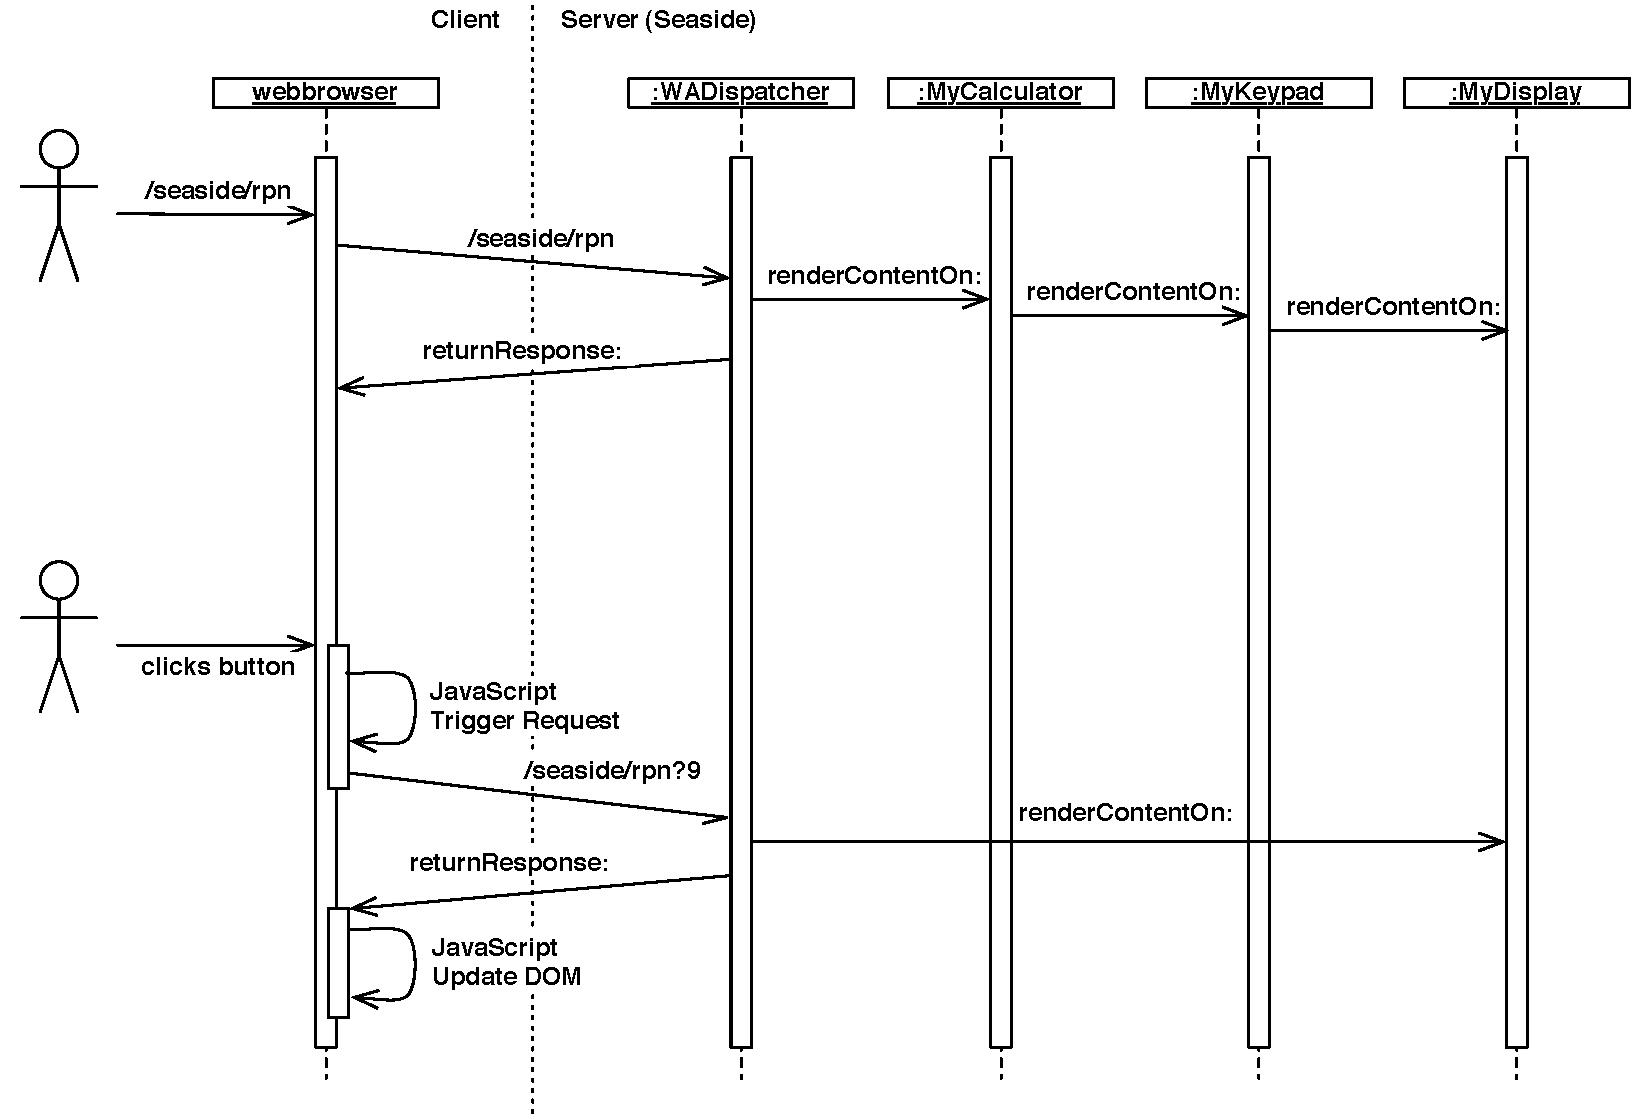
\includegraphics[width=\textwidth]{ajax-processing}
\caption{Seaside AJAX processing (simplified)}
\figlabel{ajax-processing}
\end{center}
\end{figure}

\dothis{Try the revised application.  Note that the feedback is much more natural. In particular, a new URL is not generated with each keystroke.}

You may well ask, \emph{yes, but how does this work?}
\figref{ajax-processing} shows how the RPN applications would both without and with AJAX.
Basically AJAX short-circuits the rendering to \emph{only} update the display component.
Javascript is responsible both for triggering the request and updating the corresponding DOM element.
Have a look at the generated source-code, especially the JavaScript code:

\begin{code}{}
new Ajax.Updater(
	'display',
	'http://localhost/seaside/RPN+Calculator',
	{'evalScripts': true,
	  'parameters': ['UNDERSCOREs=zcdqfonqwbeYzkza', 'UNDERSCOREk=jMORHtqr','9'].join('&')});
return false
\end{code}

For more advanced examples, have a further look at \url{http://localhost:8080/seaside/tests/scriptaculous}.

\paragraph{\emph{Hints.}}
In case of server side problems use the Smalltalk debugger.
In case of client side problems use FireFox (\url{http://www.mozilla.com}) with the JavaScript debugger FireBug (\url{http://www.getfirebug.com/}) plugin enabled.

%=================================================================
\section{Chapter summary}

\begin{itemize}
  \item The easiest way to get started is to download the ``Seaside One-Click Experience'' from \url{http://seaside.st}
  \item Turn the server on and off by evaluating \ct{WAKom startOn: 8080} and \ct{WAKom stop}.
  \item Reset the administrator login and password by evaluating \ct{WADispatcherEditor initialize}.
  \item \menu{Toggle Halos} to directly view application source code, run-time objects, CSS and XHTML.
  \item Send \ct{WAGlobalConfiguration setDeploymentMode} to hide the toolbar.
  \item Seaside web applications are composed of components, each of which is an instance of a subclass of \ct{WAComponent}.
  \item Only a root component may be registered as a component. It should implement \ct{canBeRoot} on the class side. Alternatively it may register itself as an application in its class-side \ct{initialize} method by sending \ct{self registerAsApplication:} \emph{application path}.
  If you override \ct{description} it is possible to return a descriptive application name that will be displayed in the configuration editor.
  \item To backtrack state, a component must implement the \ct{states} method to answer an array of objects whose state will be restored if the user clicks the browser's ``back'' button.
  \item A component renders itself by implementing \ct{renderContentOn:}.
  The argument to this method is an XHTML rendering \emph{canvas} (usually called \ct{html}).
  \item A component can render a subcomponent by sending \ct{self render:} \emph{subcomponent}.
  \item XHTML is generated programmatically by sending messages to \emph{brushes}. A brush is obtained by sending a message, such as \ct{paragraph} or \ct{div}, to the html canvas.
  \item If you send a cascade of messages to a brush that includes the message \ct{with:}, then \ct{with:} should be the last message sent.
  Thw \ct{with:} message sets the contents \emph{and} renders the result.
  \item Actions should appear only in callbacks.
You should not change the state of the application while you are rendering it.
  \item You can bind various form widgets and anchors to instance variables with accessors by sending the message \ct{on:} \emph{instance variable} \ct{of:} \emph{object} to the brush.
  \item You can define the CSS for a component hierarchy by defining the method \ct{style}, which should return a string containing the style sheet.
  (For deployed applications, it is more usual to refer to a style sheet located at a static URL.)
  \item Control flows can be programmed by sending \ct{x call: y}, in which case component \ct{x} will be replaced by \ct{y} until \ct{y} answers by sending \ct{answer:} with a result in a callback.
  The receiver of \ct{call:} is usually \ct{self}, but may in general be any visible component.
  \item A control flow can also be specified as a \emph{task}\,---\,a instance of a subclass of \ct{WATask}. It should implement the method \ct{go}, which should \ct{call:} a series of components in a workflow.
  \item Use \ct{WAComponents}'s convenience methods \ct{request:}, \ct{inform:}, \ct{confirm:} and \ct{chooseFrom:caption:} for basic interactions.
  \item To prevent the user from using the browser's ``back'' button to access a previous execution state of the web application, you can declare portions of the workflow to be a \emph{transaction} by enclosing them in an \ct{isolate:} block.
\end{itemize}
%-----------------------------------------------------------------

%=================================================================
\ifx\wholebook\relax\else 
   \bibliographystyle{jurabib}
   \nobibliography{scg}
   \end{document}
\fi
%=================================================================
